
% arara: pdflatex: {synctex: yes, action: nonstopmode}
% arara: pdflatex
% arara: bibtex
% arara: pdflatex
% arara: pdflatex
% arara: nomencl
% arara: pdflatex: {synctex: yes, action: nonstopmode}

%\documentclass[a4crop]{ntnuthesis}
\documentclass{ntnuthesis}
\usepackage{amsmath} %equations and spacings
\usepackage[utf8]{inputenc}  %utf-8
% \usepackage{glossaries}
\usepackage{csquotes}
\usepackage{lipsum} % acces to random text
%graphics
\usepackage{graphicx}
%\usepackage[demo]{graphicx}
%caption styles
\usepackage[small,bf]{caption}
%\usepackage{caption}
\usepackage[labelformat=simple]{subcaption}
\renewcommand\thesubfigure{(\alph{subfigure})} % see subcaption doc
%<<byman
\usepackage{colortbl}
\usepackage{color}
\usepackage{sidecap}
\usepackage{enumitem}

% To include PDFs
\usepackage[final]{pdfpages}

\usepackage[table,xcdraw]{xcolor}
%byman>>

%<<byman
%% We want UK-english hyphenation patterns.byman
\usepackage[english]{babel}
\raggedright
%byman>>

%Remove Paragraph indenting
\setlength{\parindent}{0.0in}
\setlength{\parskip}{0.1in}

\setlist{nosep}

%<<byman
%% Use scalable, PostScript Type 1 versions of the Computer Modern fonts.
\usepackage{type1cm}
%% Replace the standard Computer Modern Typewriter font LaTeX uses
%% for monospace text with the PostScript font Adobe Courier.
\usepackage{courier}
\usepackage[T1]{fontenc}
\usepackage{ae,aecompl}
\usepackage{times}
%% Redefine the font used for the section headings to
%% Helvetica-Narrow Bold.
\usepackage{sectsty}
\allsectionsfont{\usefont{OT1}{phv}{bc}{n}\selectfont}
% for colour shades in tables
\usepackage{colortbl}
 %to control the title formating and spaces around the titles
\usepackage{pdfpages}
\usepackage[compact]{titlesec}
%%byman>>

%spaces under sections
\usepackage[compact]{titlesec}
\titlespacing{\section}{0pt}{*0}{*0}
\titlespacing{\subsection}{0pt}{*0}{*0}
\titlespacing{\subsubsection}{0pt}{*0}{*0}
%fonts
 %\usepackage[T1]{fontenc} %gives light font
 %\usepackage[light,math]{iwona}

%Abbreviations or Acronyms
%\usepackage[intoc]{nomencl}
% \usepackage{nomencl}
% \renewcommand{\nomname}{List of Abbreviations}
% \makenomenclature

\makeatletter
\renewcommand\chapter{\thispagestyle{plain}%
\global\@topnum\z@
\@afterindentfalse
\secdef\@chapter\@schapter}
\makeatother 

%Bibliography
%\usepackage{url}
\usepackage{natbib}%\usepackage[sectionbib]{natbib}
\usepackage{chapterbib}
%\bibpunct[:]{(}{)}{;}{a}{}{,} %citation structure
\bibpunct{(}{)}{,}{a}{}{;}
%\bibpunct{[}{]}{,}{a}{}{;}
%\bibpunct{(}{)}{;}{a}{}{,} % to follow the A&A style
%\usepackage{chapterbib}
\usepackage{hyperref}
%\hypersetup{colorlinks=true,citecolor=blue}
\hypersetup{colorlinks=true,citecolor=blue,linkcolor=blue,urlcolor=blue}

%To change box color around the links and citations, you have these other options :
%\hypersetup{citebordercolor=Violet,filebordercolor=Red,linkbordercolor=Blue}

\newcommand{\cmt}[1]{}%inline comment

%tabularx
\usepackage{tabularx}
\usepackage{tabulary}
\usepackage{longtable} %table on several pages
\usepackage{booktabs}

%<<byman
\usepackage{multirow}
\usepackage{dcolumn}
\newcolumntype{d}{D{.}{.}{-2}}
\newcommand{\tabincell}[1]{\begin{tabular}{c}#1\end{tabular}}
\newcommand{\tabincellt}[1]{\begin{tabular}{l}#1\end{tabular}}
\newcommand{\merge}[1]{\multicolumn{1}{c}{#1}}

\usepackage{array}
\newcommand{\PreserveBackslash}[1]{\let\temp=\\#1\let\\=\temp}
\newcolumntype{C}[1]{>{\PreserveBackslash\centering}p{#1}}
\newcolumntype{R}[1]{>{\PreserveBackslash\raggedleft}p{#1}}
\newcolumntype{L}[1]{>{\PreserveBackslash\raggedright}p{#1}}

% Used to create tables with rows/cols spanning over se
%% Use fancy chapter headers, with Jos Dingjan's modifications,
%% plus my own tweaks. This style is not part of teTeX,
%% so we are using a local (and renamed) copy.
%\usepackage[Lenny]{fncychapleo}
\usepackage{fncychap}

%% Nicely format and linebreak URLs in the bibliography (and elsewhere).
%%\usepackage{url}
%% Define a new 'leo' style for the package that will use a smaller font.
\makeatletter
\def\url@leostyle{%
  \@ifundefined{selectfont}{\def\UrlFont{\sf}}{\def\UrlFont{\small\ttfamily}}}
\makeatother
%% Now actually use the newly defined style.
\urlstyle{leo}
%byman>>

%graphics
\usepackage{epstopdf} %support for eps.
\DeclareGraphicsExtensions{.eps,.ps,.pdf,.png,.jpg}
\usepackage{float} % figure placing [H]

%landscape Option
\usepackage{lscape} %Left down
%usepackage{pdflscape} %Left up)

\usepackage[draft]{todonotes}   % notes showed (JJUNJU)
% Select what to do with command \comment:
% \newcommand{\comment}[1]{}  %comment not showed
\newcommand{\comment}[1]
{\par {\bfseries \color{red} #1 \par}} %comment showed

%Section Numbering and TOC depth
\setcounter{secnumdepth}{2}
\setcounter{tocdepth}{1}

%chapter biblio
\usepackage{chapterbib}

%Drawing flow charts
\usepackage{tikz}
\usetikzlibrary{shapes,arrows}
\tikzstyle{decision} = [diamond, draw, fill=blue!20,
    text width=4.5em, text badly centered, node distance=3cm, inner sep=0pt]
\tikzstyle{process} = [rectangle, draw, fill=blue!20,
    text width=5em, text centered, rounded corners, minimum height=4em]
\tikzstyle{line} = [draw, -latex']
\tikzstyle{output} = [trapezium,draw, trapezium left angle=70,trapezium right angle=-70,fill=pink, text width=3em, minimum height=2em,text centered]
\tikzstyle{data} = [trapezium,draw, trapezium left angle=70,trapezium right angle=-70,fill=white!20, text width=3em, minimum height=2em,text centered]
\tikzstyle{space} = [rectangle, fill=white,opacity=0,text width=5em, text centered, rounded corners, minimum height=4em]
\tikzstyle{results} = [ellipse,draw,fill=white, text width=4em, minimum height=3em,text centered]

%To generate list of symbols
\newcommand{\addsymbol}[3]{%
  \symboldisplay{#1}{#2}\\%
  \setelem{#3}{#1}
}
\newcommand{\symboldisplay}[2]{%
  $#1$ \parbox{5in}{\dotfill #2}%
  %$#1$ \parbox{5in}{ #2}%
}
%\def\setelem#1{\expandafter\def\csname myarray(#1)\endcsname}
\def\setelem#1{\expandafter\gdef\csname myarray(#1)\endcsname}
\def\dispsymbol#1{\csname myarray(#1)\endcsname}

% \makeglossaries
 
% \newglossaryentry{latex}
% {
%     name=latex,
%     description={Is a mark up language specially suited 
%     for scientific documents}
% }
 
% \newglossaryentry{maths}
% {
%     name=mathematics,
%     description={Mathematics is what mathematicians do}
% }


%Titles
\title{AnyBoard game platform}
\subtitle{A software platform supporting the development of hybrid board games that uses IoT devices.}
\author{Tomas Albertsen Fagerbekk}

\def \thesisAuthor{Tomas Albertsen Fagerbekk}

\degreetype{Master}
\faculty{Faculty of Information Technology, Mathematics and Electrical Engineering}
\department{Department of Computer and Information Science}
\setyear{2015}
%\setmonth{Desember}

\begin{document}

\frontmatter
\maketitle

\chapter{Abstract}
Previous work has sparked interest in hybrid games, games that combine video games and traditional board games by using digital surfaces or tangible, digital tokens. Whilst video games provide a rich, dynamic and interactive environment, board games has the advantage of a social face-to-face interaction. Hybrid board games attempts to combine the best of both, providing the dynamic interactivity of digital games with the social aspect of traditional games.

In this thesis a software platform has been made for creating hybrid board games. The goal was to simplify the challenges with creating and implementing game concepts digitally, in combination with integrating tangible digital devices.

The work has resulted in AnyBoard, a JavaScript based platform that is openly available at \href{https://github.com/tomfa/anyboardjs/}{github.com/tomfa/anyboardjs}. A common communication protocol as well as firmware implementations for two different arduino-based chipsets has been developed and tested on mobile surfaces. With the current state of the AnyBoard platform, developers are able to create games using pawns that detect location, display colors and print cards from a mobile-surface game hub, without knowing anything but common web technology. The platform supports integration with any other JavaScript-based game engine or game development tool available.

AnyBoard can be used as is to create hybrid board games, but also has a great potential to become a richer and more potent tool by further implementation.


\textbf{Keywords: hybrid games, board game, tangible interfaces, internet of things, iot}
\newpage
\chapter{Preface}
This project was carried out as a Master’s thesis at NTNU as part of the MSc programme in Computer Science during the summer of 2015. The work has been supervised by Monica Divitini and co-supervised by Simone Mora.

The work is in large part motivated by challenges with previous projects done by students of supervisor Monica Divitini when creating hybrid board games. The contributions from the student include the development and design of the AnyBoard library, token drivers and firmware that is located at \href{https://github.com/tomfa/anyboardjs/}{github.com/tomfa/anyboardjs}. Available open source libraries and modules have been used where applicable.

The design and assembly of the arduino-based tokens has been done by co-supervisor Simone Mora.

Thanks to my supervisors for guidance, input and motivation throughout the thesis. You've been great!

\newpage


%% Configuration of the header strings for the frontmatter pages.
\fancyhead[RO]{{\footnotesize\rightmark}\hspace{1em}\thepage}
\fancyhead[LE]{\thepage\hspace{1em}\footnotesize{\leftmark}}
\fancyhead[RE,LO]{}
\fancyhead[RO]{{\footnotesize\rightmark}\hspace{1em}\thepage}

%TOC
\tableofcontents
%\addcontentsline{toc}{chapter}{Contents}

%\listoftables
%\addcontentsline{toc}{chapter}{List of Tables}

\newpage
%\listoffigures
%\addcontentsline{toc}{chapter}{List of Figures}

%Abbreviations

%\thispagestyle{empty}
% \printnomenclature
%\cleardoublepage

%Symbols
%\newpage
%\chapter*{List of Symbols\hfill}
%\addcontentsline{toc}{chapter}{List of Symbols}
%\begin{flushleft}
%   \input{symbols}
%\end{flushleft}
 
% \printglossaries

\mainmatter
\chapter{Introduction} \label{ch:introduction}
The aim of this thesis is to look at how one can simplify the development of hybrid board games.
The next sections of this chapter describe the context and motivation of the thesis. The research
questions and research method are also described. The final section, \ref{sec:introoutline}, gives an outline of the report.

\section{Motivation} \label{sec:motivation}

\subsubsection{Hybrid board games are more immersive and than traditional board games}
The limitations of traditional board games lies in the static tokens and constrains. It is up to the players to understand the concepts and rules, as well as imagine or enforce the consequences of their actions. A digital game on the other hand is more dynamic with a richer interface which can be more absorbing. Consequences of a players actions can be enforced and accompanied by sound, vibration and graphical simulation. But digital games often take focus away from the social aspect of their traditional counterparts.

The hope for hybrid board games is an immersive, dynamic game play that also keeps the social aspect of face-to-face interaction.

Previous work on hybrid board games has been done both at NTNU with Don't  Panic\cite{di2012don} and in other projects\cite{al2008designing, bakker2007weathergods} showing good results.

One comparison between tabletop and traditional board games even indicate that "senior citizens found the tabletop version of the game to be more immersive and absorbing [than regular board games]"\cite{al2008designing}.

\subsubsection{Existing tools can be difficult to set up}
In the testing of Don't Panic\cite{di2012don}, the users enjoyed the game play and showed enough interest in the game to request to keep a version of the game. The challenge with this was the complexity of setting the game up. It required turning on an off-site server that held a database and worked as a sort of game hub, as well as manually starting scripts in on-site components. The result was that it wasn't feasible for the players to initialize the setup of the board game by themselves. 

In addition to this, much time had been put into programming the devices. Creating a replica of the game required much more than ordering a new set of hardware.

\subsubsection{Existing tools can be expensive}
In other more established tools for hybrid board games, the interaction is typically done via tabletop devices\cite{al2008designing}, such as Microsoft Surface Hub\footnote{\href{https://www.microsoft.com/microsoft-surface-hub/en-us}{www.microsoft.com/microsoft-surface-hub/en-us}}. These devices, similar to a table with a large touch screen on top, restrict the mobility of the game, require a dedicated physical space and remain a large investment in terms of money.

\subsubsection{Creating hybrid board games is time consuming}
While there are plenty tools for creating online games, and a few for creating hybrid tabletop-based games, we have been unsuccessful in finding existing tools for creating hybrid board games that uses small hardware tokens. 

The result when implementing Don't Panic was creating custom scripts and communication for the different pawns and implementation of game logic. Needless to say, this was very time consuming.

\section{Problem definition}
Based on the observations made in the previous section, we see that hybrid board games pose several problems.

The cost for developers to develop new hybrid board games is terms of time is very big. They are required to create most of their game from scratch, as there are few suitable existing tools. Due to the different types of components in a hybrid game, they will also have to know several kinds of technology.

Also in terms of money, the cost for developers is big. Due to the lack of standard tools, creating a game that makes use of a certain token\footnote{\emph{Token}: A term we will use in this thesis a lot to note a tangible piece of hardware used in a hybrid game. E.g. a digital pawn.} will require acquiring that token, since one cannot be certain it works without actual testing.

For players, the acquisition cost for the required hardware is huge if we consider the tabletop solutions. If we on the other hand consider hybrid games with tokens, the lack of mature software solution require players to have time and technical knowledge to set up and use.

% \begin{itemize}
% \item{The cost for developers to develop new hybrid board games in acquiring hardware and software tools should be a minimum}
% \item{The time invested by developers to learn new languages and tools, should be kept to a minimum}
% \item{Developing the game should be de-coupled from the tangible hardware used during playing, so that a game can be replicated easily for different types of hardware.}
% \item{For players, the acquisition cost for the required hardware should be as low as possible}
% \item{For players wanting to play such games, it should be easy and quick to initializie the hybrid games.}
% \end{itemize}


% Not sure where or if to include this
%
%\subsection{How digital interfaces enhance the experience of playing a board game}
%\subsubbsection{A larger library of events}
% A digital board game can hold a larger library of cards, colors and events, as a digital object is  dynamic. A pawn can be of different colors depending on the situation. A screen can show different cards.
%
%\subsubsection{Simplify introduction to the game}
% A digital tool can describe the game in a richer way (through video, sound) and provide greater help (faq, integrated forums) than traditional paper manuals.
%
%\subsubsection{Simplify modification and updates}
%Modification of a digital board game can become as easy as clicking and update button, or selecting a different mode.
%
%\subsubsection{Encourage creating of own games}
%An open source board game kit with hardware components and an open API is can encourage hobbyentusiast and game interested developers to create their own games.
%
%
\section{Research questions}

Below are our research questions. The first being a main question, that embraces those that follow.

\textbf{RQ1: How can we lower the barrier for developers to start creating hybrid board games?}
We do wish for as many as possible to start creating hybrid board games. In order to get there, we need to lower the barrier so that more developers play around with the technology and get interested.

\textbf{RQ2: How can we lower the investment required by developers, both in time and money, in order to create hybrid board games?}
One of the main obstacles we have seen from previous work is the amount of time involved. If creating hybrid board games was quick and cheap, more developers would do the same.

\textbf{RQ3: How can we facilitate developers so that they are able to simplify the setup of such board games, in order to make it easy for players to acquire and play hybrid games?}
We believe in the importance of involving non-technical people in these games. If developers are able to create hybrid board games that \emph{everyone} is able to set up and use, this opens a range of new possibilities, including creating a business around it.

\section{Research method}
This thesis takes an experiment approach to developing a platform for creating hybrid board games. Due to practical reasons, adjustments to the development process and requirements has come by evaluation from ourselves, without feedback from outside user groups.

The process led to the creating of a platform, to address challenges from previous work done with hybrid games. First by review of relevant literature and current workflow for creating these games. This was followed by a design process and implementation phase, before we evaluated how the resulting platform addressed the identified challenges.

\section{Contribution}
This thesis has resulted in a AnyBoard, a JavaScript-based platform for creating hybrid board games. It is openly available on \href{https://github.com/tomfa/anyboardjs}{github.com/tomfa/anyboardjs}.

The location also includes extensive documentation, several examples, tests, and drivers as well as firmware for three different tokens. These are also described in appendix \ref{appendix:doc}, \ref{appendix:examples}, \ref{appendix:tests} and \ref{appendix:tokens} respectively. For the source code itself, we refer to the Github repository in the previous paragraph.

The thesis has already formed the basis for a published article from our institute, \emph{Making interactive board games to learn: Reflections on AnyBoard}\cite{anyboard_article}. This article is included in appendix \ref{appendix:article}

In addition, we'd like to point to the Future work in chapter \ref{sec:future_work} where we suggest different directions and features for  AnyBoard to continue.

\subsection{Limitations}
AnyBoard itself is compatible with any JavaScript-environment. As such, it can be integrated with any other JS-framework or game engine without issues. For communication with tokens, AnyBoard depends on plugin-drivers with a firmware compatible with that driver. These drivers can pose their own limitations.

The drivers and firmware for three types of tokens we have made, can be seen in appendix \ref{appendix:tokens}. These require Evothings bluetooth libraries and Cordova libraries. This limits their use to Android and iOS environments. 

\section{Thesis outline} \label{sec:introoutline}
Here we describe the structure of the report. The report is split into seven section.

The first section (chapter 1) consists of the introduction to and motivation for this thesis and the work that has been done. We explain the why, what and how of the thesis, providing a problem definition, research questions and method.

Section two (chapter 2) contains a problem elaboration. We take a look at previous related work, and characteristics of common board games as well as what concepts they include. A description of the life cycle of developing hybrid board games and which roles are involved follows, and thereafter we identify common challenges AnyBoard should address. We then illustrate a rough outline of the platform and the parts it should consist of, before we finally present a set of high level requirements for AnyBoard.

In the third section (chapter 3), we evaluate different tools and platforms for AnyBoard to make use of or build upon. Creating a hybrid digital game is a complex process, and here we look at existing tools that can be used in collaboration to simplify the complexity and make use of existing communities.

The fourth section (chapter 4-5) involves the design and implementation of AnyBoard. We present non-functional and functional requirements in section \ref{sec:requirements}, followed by a more specific architecture for AnyBoard. In chapter \ref{ch:implementation} we present the implementation. Details on the parts that was developed, the game entities and token communication protocol among other things. 

Evaluating the result is done in the fifth section (chapter 6). We implement two common game concepts, both with and without the use of AnyBoard. First, we "draw" cards from a deck, represented by a printer. Secondly, we answer a quiz by moving tokens on fields representing alternatives. We evaluate how AnyBoard made this easier, and compare it to the implementation without the use of AnyBoard.

Lastly (chapter 7), we summarize and discuss the what could've been done better. Which parts of the thesis gave value and not. We explain what this mean for our research questions, before we provide our suggestions and thoughts around future work.
\newpage

\chapter{Problem Elaboration}

\section{Previous work}
This thesis and its motivation derived from previous work with hybrid games at NTNU, as mention in chapter \ref{ch:introduction}. In particular, Don\'t Panic was well received, but implementation was time consuming and setup during play proved difficult for players\cite{di2012don}. 

Other work done regarding hybrid games are often centered around tabletops\footnote{With \emph{tabletop} we refer to a table computer, such as Microsoft Surface 1.0 or Samsung SUR40} as the central component of the game. Weathergods\cite{bakker2007weathergods}, KnightMage\cite{magerkurth2004towards} and False Prophets\cite{mandryk2002false} are examples of these. Most of these report a positive feedback from users, inclining that hybrid games indeed can utilize the best from both regular and digital games. An article evaluating tabletop game experience for seniors even claim they enjoy hybrid games and get more immersed than with regular games \cite{al2008designing}.

Two framework has been previously developed for creating tabletop board games: ToyVision\cite{marco2012toyvision} and ReacTIVision\cite{kaltenbrunner2007reactivision}. However, their relevance might be dwindling, as tabletops for private use has near to disappeared. Most of the existing work regarding tabletop games was done in the period 2004-2010. Since then, there has been little development around tabletop games and tabletops in general, at least that target to the private consumer marked. Microsoft PixelSense\footnote{Microsoft PixelSense: Microsofts initative for tabletops.}, and their accompanied hardware, Samsung SUR40 is retired, according to their own websites\footnote{\href{http://www.samsung.com/uk/business/business-products/smart-signage/specialised-display/LH40SFWTGC/EN}{www.samsung.com/uk/business/business-products/smart-signage/specialised-display/LH40SFWTGC/EN} displays Samsung SUR40 as no longer available.}. We speculate that the high cost of aqcuiring tabletop devices\footnote{Samsung SUR40 currently goes for about 5000 USD on eBay market} has played a large role.

Hybrid games without tabletops has also been created. The game \emph{"In Search of the Amulet"}\cite{magerkurth2012hybrid} an 8x8 tiled board  implemented with rfid tags was used together with rfid readers inside digital player pawns. The pawns detected its movement and location on the board, and reported it to a computer. Each player here had each their computer functioning as a private space and allowing them to do actions without the other player knowing. In addition, a "public" screen showed information visible for both players. One of the challenges here was the potential intruising effects of the displays, and it was deliberately made to require as little as possible interaction with the digital components in order to uphold the social aspect. The article does not mention any hybrid game platforms being used.

\subsection{Summary}
Hybrid games of various kinds has been tested, prototyped and developed previously. From those articles we've seen, there has been nothing but  positive feedbacks from users, who have found such games entertaining and immersive.

Platforms for developing hybrid games more easily has been made, but these are centered around tabletop environments, which is not suitable for our task, due to their high aqusition cost.

With the exception of \emph{In Search of the Amulet}\cite{magerkurth2012hybrid}, we've been unable to find previous work of hybrid games with simple digital pawns independant of a tabletop device. We have been completely unable to find hybrid game platforms similar to the one we've planned to develop.

\section{Characteristics of board games} \label{sec:boardgames_commonalities}

In this section we will analyse three different board games to identify and classify typical components of the board games. The purpose of this is to identify classic types of interactions and components in board games, so that we can focus on the central elements to implement in our platform. 

At the end we summarize the elements we've identified. The characteristical concepts of board games are described in subsection \ref{subsubsec:boardgame_concepts}, while the physical components common for board games can be found in subsection \ref{subsubsec:boardgame_components}. 

The three board games we've chosen is Lords of Waterdeep, Monopoly and Don't Panic. These are chosen to cover common, but different types of board games. Lords of Waterdeep is a classic Dungeons and Dragons game, making use of typical "advanced" board game dynamics, while Monopoly is a simpler common type of board game, employing many standard actions and elements. Don't Panic has been chosen as an existing hybrid board game.

\subsection{Monopoly}
Monopoly is a widely popular property trading game. Players acquire properties and money through chance cards, landing on property tiles and completing "laps" on the board. They charge each other money for the "use" (landing on) their land. Players lose by going "bankrupt", which is when their assets amount to less than 0 amount of money. The \textbf{winner is declared when} all other players are bankrupt.

\begin{figure}[ht]
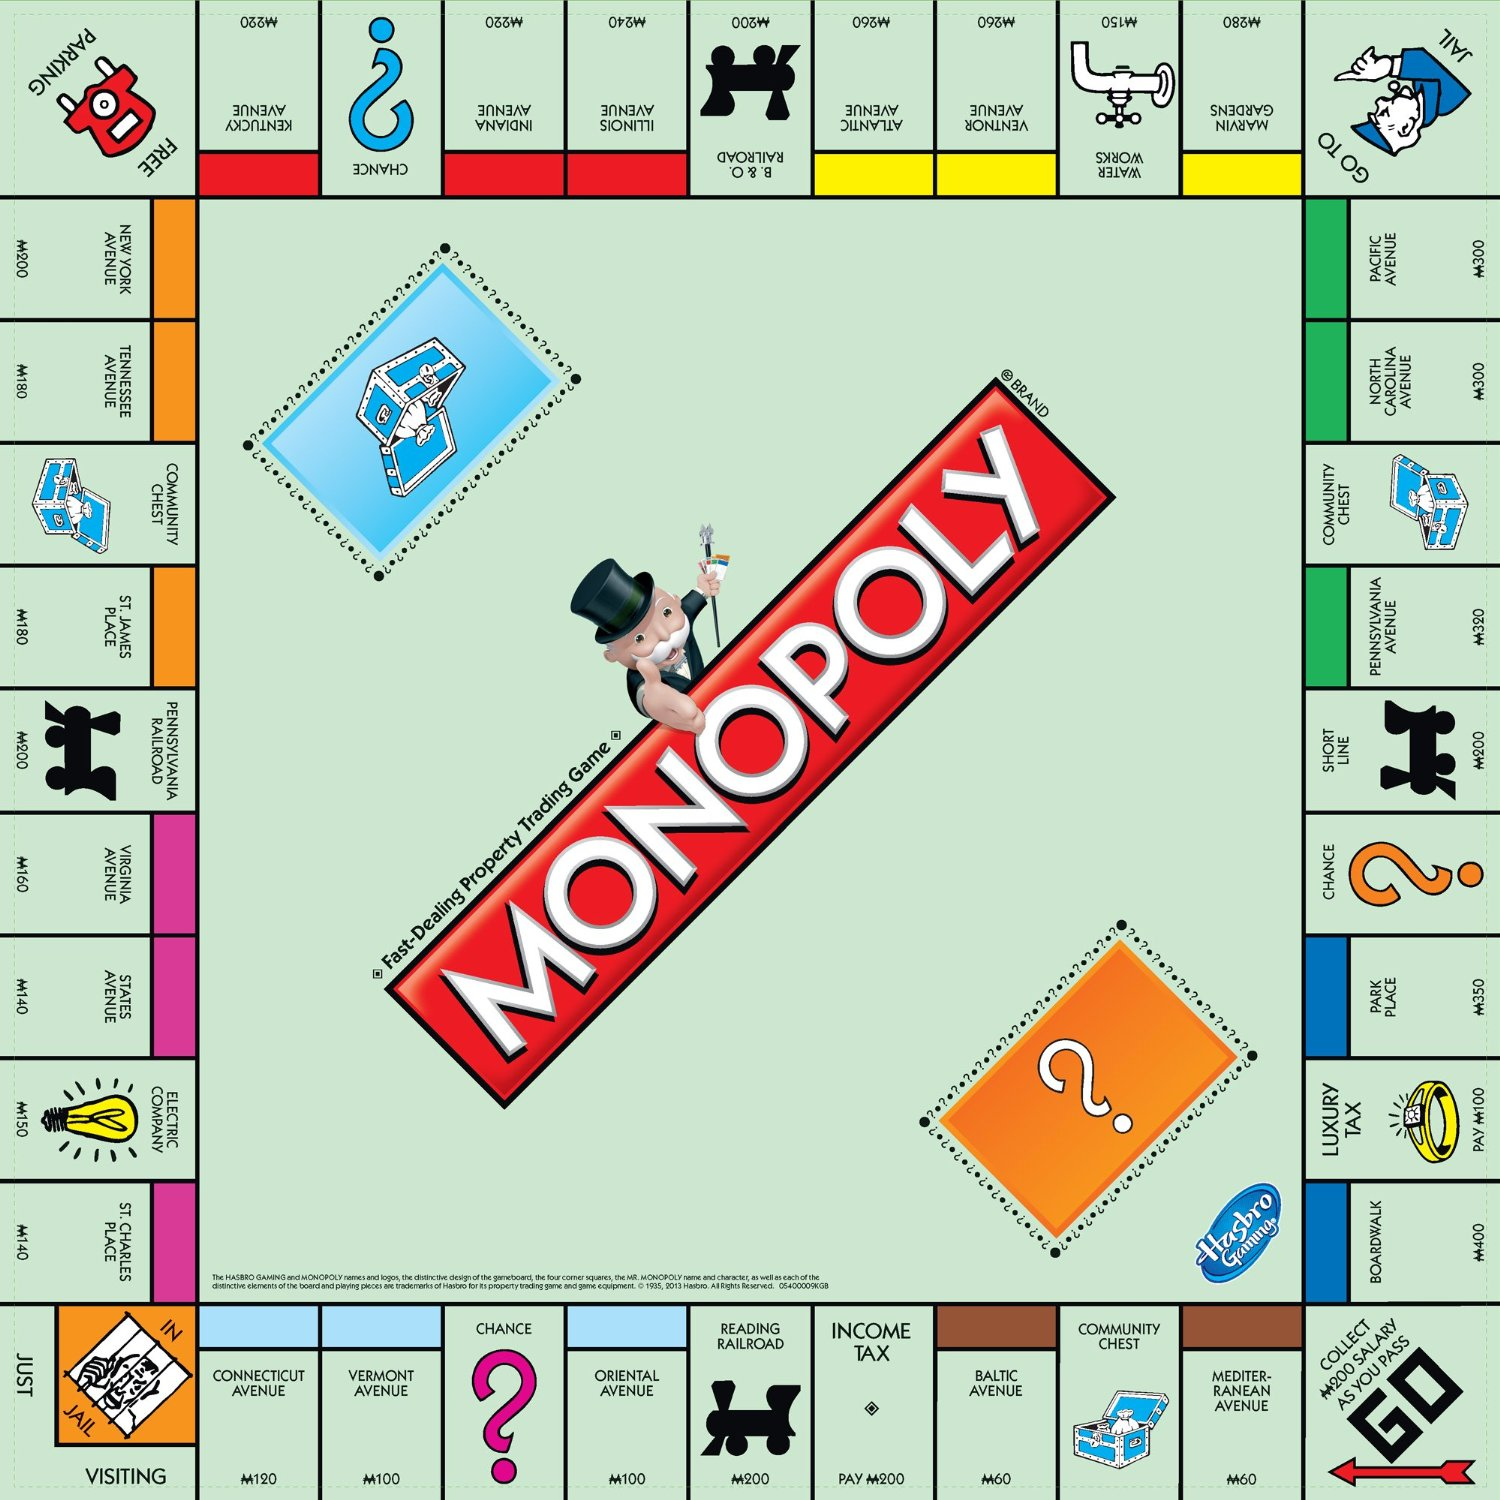
\includegraphics[width=12cm]{img/monopoly_board}
\centering
\caption{A version of Monopoly from Parker Brothers. Player pawns move from one to the next of the 40 tiles clockwise using two six sided dices.}
\label{fig:monopoly_board}
\end{figure}

The Monopoly \textbf{board} consists of roughly 40 discrete \textbf{tiles} as shown in figure \ref{fig:monopoly_board}. Each player has a \textbf{pawn} that represents them, which they move about the board with. The movement is determined by a roll of \textbf{dices}. Monopoly is \textbf{turn-based}, which means players take turn to throw the dices, moving their pawns, and completing a set of possible \textbf{actions} they can choose from, determined from the tile they land on. 

Each action usually involves buying, paying or exchanging  \textbf{resources} in form of money or stocks – which are placed in an inventory of each player. The inventory is a \textbf{private space} which contains the resources belonging to that player. Players starts the game with some initial resources in their inventory, but most are acquired during the game play. Resources are represented in form of two sorts of \textbf{informational tokens}: stocks and monopoly money. 

In short, the goal of the game is to maximize the acquisition of resources.

\subsection{Lords of Waterdeep} \label{subsec:LoW}
Lords of Waterdeep (LoW) is a \textbf{turn-based} game from the Dungeons and Dragons series, where players fight as a Lord in order to control a city. The goal of the game is to maximize the number of \textbf{points}. which are obtained mainly by completing quests. Quests are completed by obtaining a spesific combination of different adventureres in addition to a quest-card. 

In addition to quests and resources held by a player (marked red in figure \ref{fig:lords_board}), each player also is a spesific Lord (\textbf{Role}) which gives bonus points to certain quests for that player. LoW also include a type of cards called Intrigue, which can be used in various advantageous ways.

\begin{figure}[ht]
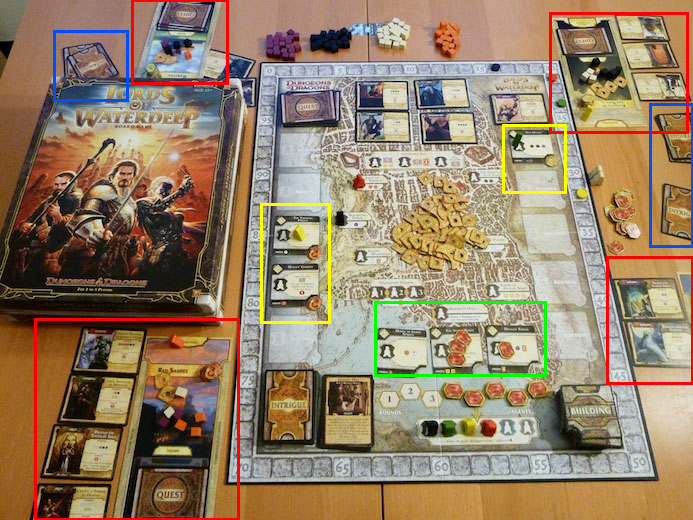
\includegraphics[width=12cm]{img/lords_board_marked}
\centering
\caption{Lords of Waterdeep. Players have multiple pawns and place them on available tiles as they please. New tiles (yellow) can be bought into the game allowing for a greater set of possible actions. Each player has both a visible (red) and hidden (blue) private space.}
\label{fig:lords_board}
\end{figure}

The Lord and Intrigue-cards are held in a \textbf{hidden private space}, a space that is not visible to other players other than the holder. Compared to games that doesn't have such dynamic, this hidden space introduces a new dimension to the game, as players hold different information.

LoW also make use of \textbf{rounds}. After all players have placed their pawns on the board, and actions has been completed, a round is over. All pawns are being put back into the inventory of each player, and points given by acquiring new tiles (buildings) are increased. After the fourth round, players are given an extra pawn, and the game ends after the eight round.

Another interesting component of LoW is its \textbf{dynamic board}. Of of the initial tiles can be used by players that wish to buy a new tile. The new tile will be an available in that and all the remaining rounds, and will reward the buyer upon usage.

\subsection{Don't Panic}
Don't Panic (DP) is a \textbf{cooperative} board game with different zones, where panic can emerge among "people" and spread to nearby zones. The players, unlike in Monopoly or LoW, work together in an effort to reduce panic. In DP, the players attempt to calm a situation down, and loses if the panic level goes beyond a certain threshold.

\begin{figure}[ht]
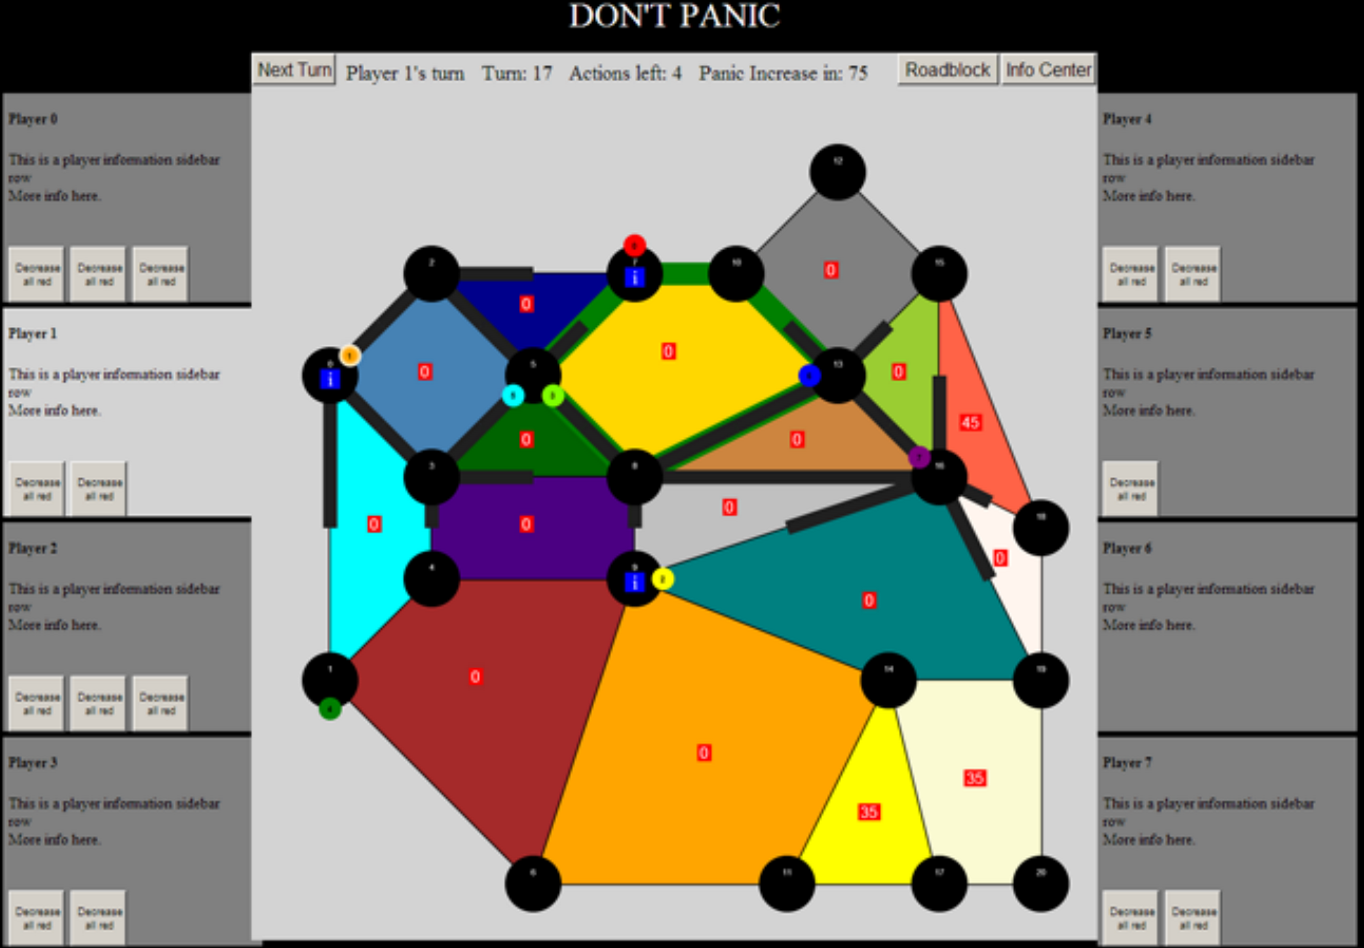
\includegraphics[width=12cm]{img/dont_panic_interface}
\centering
\caption{Digital version of Don't Panic. The map is divided into zones with a respective panic level. Player pawns locate themselves on the different nodes, and attempt to lower and contain the panic.}
\label{fig:dont_panic_board}
\end{figure}

Each player is presented by a pawn (colored circles in figure \ref{fig:dont_panic_board}) located on tiles (black nodes), and takes turn to draw 2 informational cards, 2 event cards and complete 4 "actions". Event cards are challenges which the players have to deal with on their turn, and can be resolved by "actions" or the use of informational cards. The informational cards are a form of resource that can (optionally) be used on a players turn. 

The 4 "actions" performed by players on each turn can be chosen from a set of actions containing movement of pawn, movement of people between zones, set up or remove road blocks to contain panic, as well as building an information center. Each player is also randomly given a role at the start of the game, which gives them an advantage on a spesific type of action. 

Once the game starts, a \textbf{timer} is initialized, counting down from a certain amount of minutes. Once the timer rings, panic levels are increased, and can spread between zones. This introduces a dimension of stress or hurry to the game, as playing faster gives an advantage.

\subsection{Summary: concepts} \label{subsubsec:boardgame_concepts}
\textbf{Players and Teams}: Board games are typically played in social settings with two or more players. In many board games such as Monopoly, each player is represented with a physical object called "pawn". In LoW, we saw that this is not the case, but rather had several agents that acted on behalf of the player.

Commonly, every player play each against other and is as such on team with only themselves, such as in Monopoly or Low. In other games, such as DP, several or all players can also play on teams with each other, fight common enemies even including the game itself.

\textbf{Roles and skills} are player-spesific properties that deviate from the standard rules of the game, and can give advantages or disadvantages in different aspects of the game. In DP, each player is assigned a Role by random, which gives them advantages in performing certain actions. For example, a driver can move more people out of paniced areas. Similarily in LoW, each player is assigned a Lord card (character) by random, which increases the points granted upon completing certain quests. LoW also has special quests that provide an advantage for the rest of the game (skill). For example, completing the quest "Quell Merchenary Uprising" will provide the player with two extra points for every other quest of the same type he or she completes.

\textbf{Public and private spaces}: Public and private spaces are the conceptual areas containing parts of the game that is interacted with by all or one of the players. Public spaces can be interacted with by all players, while each player has a private space that only that player can interact with. In Monopoly, question cards, dices and cards are a part of the public space, while money belong to the private spaces of each player.

\textbf{Hidden private space}, is the a private space that is not visible for other players. For example a hidden hand contains cards that are visible only to the holder of the cards. For example in LoW your Intrigue cards (uncommon advantageous actions you can perform) is hidden from other players. 

\textbf{Themes} provide a background story and explain the motivation and goal for the players. Both Monopoly, LoW and DP have themes that help relate the game to real world concepts and provide some story that can help players immerse them selves in the games. This is unlike games as Poker or Tic Tac Toe.

\textbf{Events} are special parts of the game that often go outside the normal flow of the game. In Monopoly, one of the tiles will send you to "jail". This includes a movement of the pawn that is not based on dices like the rest of the game, and gives an exception to the dice rolling and movement in the next turns. An event is also triggered when drawing question cards: winning the lottery or having to repair your houses go outside the normal flow of the game. In LoW, playing Intrigue cards will trigger events, allowing for players to take resources from others or imposing a mandatory quest upon other players. And in DP, Event Cards and playing Informational Cards can be categorized as events. Events are typically unpredictable, either by being in a shuffled deck of cards or played from a hidden private space.

\textbf{Resources} are assets belonging to a player. In Monopoly, the resources are Stocks, Money and Houses. Player controlled events, such as the Get Out of Jail Free Card (Monopoly) or Intrigue card (LoW) can also be considered resources. Resources are often made physical through Indicator Tokens (see \ref{subsubsec:boardgame_components}).

\textbf{Turns and actions}: In turn-based games each player takes turn to complete some actions, before the next person plays his turn. Each turn usually involves a scripted set of actions. In Monopoly, you must always roll two dices and move your pawn that amount of tiles. This is a mandatory action. The tile determines the next set of actions you can perform. Either 1) pay the owner rent (mandatory), if the tile is currently owned by anther player, 2) buy the stock (optional) if the tile is for sale, 3) draw a card and complete it's action (mandatory) if landing on a question-tile. In other words, turns are sets of actions, where each action can either be mandatory or optional, that can have a precondition, i.e. do this if that, and can be ordered, i.e. done in a speific order.

\textbf{Rounds} is a concept that some event or set of events will incur, usually that sets back the game in some way, after some critiera is met. In LoW, actions is performed via agents, which is "spent" once put on the board. When all agent actions are exhausted, the round is over, and agents are put back into their respective players private space so that they can perform actions on behalf of the player again. In DP, one can interpret the time between each alarm as a round. Once the round is over, panic is increased and potentially spread.

\textbf{Rules} tell us the possible interactions between game components: Which actions is involved in a turn? When is a round over? How can your pawn move around the board? When is a winner declared, or a player out of the game? Rules explicitly define the starting conditions upon starting the game, and are a central part of all games, as they dictate the flow of the game and define the bounderies of them.

\subsection{Summary: Physical components} \label{subsubsec:boardgame_components}

\begin{figure}[ht]
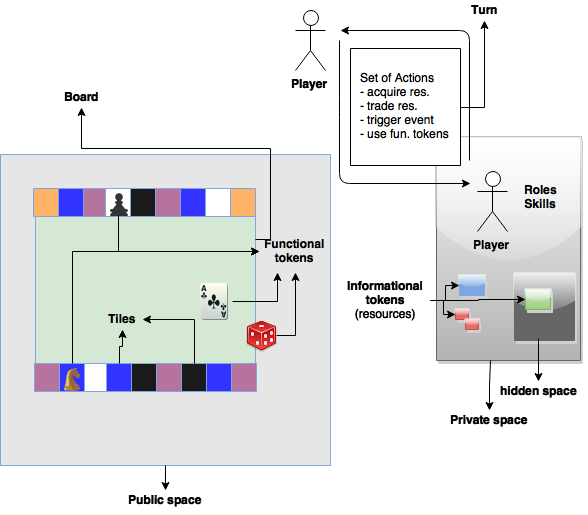
\includegraphics[width=12cm]{img/board_games_components}
\centering
\caption{Common components of board games. Board with tiles and functional tokens as a part of the public space, while informational tokens (resources) as part of each players private space, potentially hidden from view from other players. The game is progressed by players taking turn to acquire and trade resources, triggering events and interacting with functional tokens.}
\label{fig:board_games_components}
\end{figure}


\textbf{Board} is the surface used to play a board game. Most games have a unchanging board (Monopoly), while some have a modular board with varying layout in each session or while the game is played (LoW). The board consists of tiles and placeholders for other assets.

\textbf{Tiles} are discrete locations on the board. Which tile a player is located on, usually determines which set of \emph{actions} the player can perform. In Monopoly for example, a stock can only be bought when the the pawn is located on that spesific tile. In Don't Panic, it didn't determine which actions one could perform, but rather which part of the city the player could perform his actions upon. In some games, such as Monopoly and DP, movement is only allowed over adjecent tiles.

\textbf{Indicator tokens}, e.g. Gold, Wood, Stone, Gas, Money, Points, Stocks and Houses help keeping track of an informational aspect in the game. In Monopoly, the paper money is simply an indicator of how much resources owns, and stocks an indicator of the lots owner. It serves its purpose by holding some information, and as such simplifying the amount of information players have to remember and keep track of themselves.

These are simple tokens, as they are only representatational of some game information, and does not change the game state or provide interactive functionality like randomness. Such tokens can easily be replaced by a number value or position on a screen, as they are not interacted with other than changing owner.

\textbf{Functional tokens}, e.g. dice, cards and pawns play an active part in how the game unfolds. For example, a dice in provides randomness as a functionality to the player, while the timer in DP provide an aspect of time or hurry. Cards are the most common functional tokens, which can provide many types of events and exceptions to the standard flow of the game, as well as provide randomness through being shuffled and used in a drawable deck.

These tokens change the state of the game by opening or closing certain actions and aspects for players. Each of these tokens have a specialized functionality, and can not be implemented as generally as indicator tokens.

\newpage


\section{Life cycle and roles}
In this section we go through the life cycle of a game, from idea through creation to a playable augmented board game. We focus on the roles and their contributions and actions in creating and using the game, as was the case with the previous augmented board game created at NTNU, Don't Panic . In the next section we will look at the challenges linked with these activities. 

We have identified three roles: a \textbf{Game Designer}, who formalizes and defines the game. The end result from a game designers production is a playable paper prototype. A \textbf{Developer} takes this prototype and identifies and acquires suitable hardware pieces, designs the user interface to be used in the game controller and implements the game through the controller and the hardware tokens. A \textbf{Player} should then able to acquire, set up and play the game. These roles and their typical activities are illustrated in figure \ref{fig:LifeCycleGameDesigner}, \ref{fig:LifeCycleDeveloper} and \ref{fig:LifeCyclePlayer}. The activites that we will focus on in this thesis is marked in green.



\begin{figure}[ht]
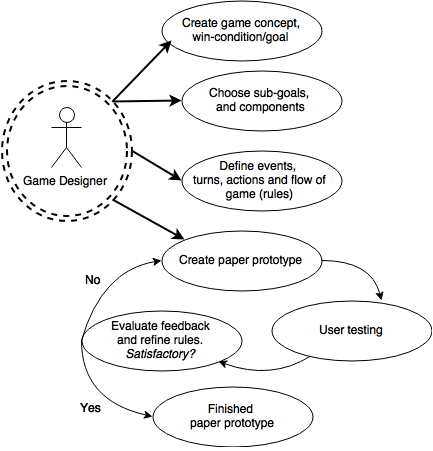
\includegraphics[width=8cm]{img/LifeCycleGameDesigner}
\centering
\caption{An overview over the responsibilities of the Game Designer in implementing hybrid board games. }
\label{fig:LifeCycleGameDesigner}
\end{figure}

\begin{figure}[ht]
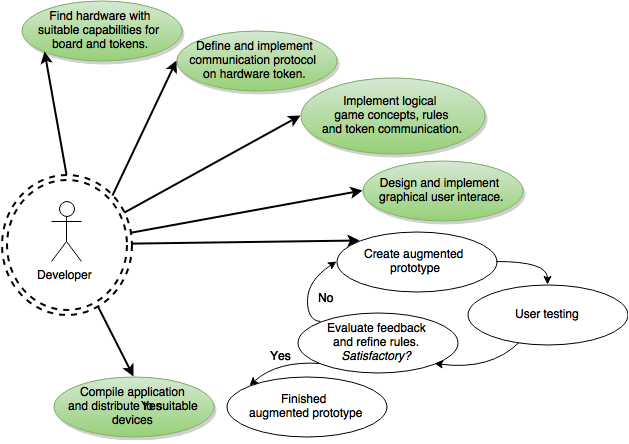
\includegraphics[width=12cm]{img/LifeCycleDeveloper}
\centering
\caption{An overview over the responsibilities of the Developer in implementing hybrid board games, after a finished paper prototype is provided by the game designer. The responsibilites marked with green are areas where we think AnyBoard can assist.}
\label{fig:LifeCycleDeveloper}
\end{figure}

\begin{figure}[ht]
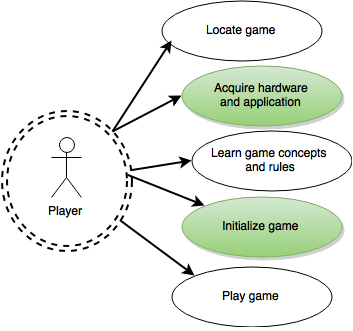
\includegraphics[width=7cm]{img/LifeCyclePlayer}
\centering
\caption{Main interactions from the view of a player in using hybrid board games. From previous experience in the testing of Don't Panic, replacing hardware tokens and game initialization (marked green) was too hard for non-technical players to receive a copy of the game.}
\label{fig:LifeCyclePlayer}
\end{figure}

\subsection{Designing}
The Game Designer starts with an idea, and details it through defining concepts, providing a motivation/goal, and giving the game clear rules and boundaries. The end result from the game designer should be a playable paper prototype of the board game. The following questions are the main questions that a game designer should be able to provide answers for (short Monopoly example answer in emphazised text):
\begin{enumerate} \label{design_cycle}
\item How are the teams - who is playing against who? \emph{Every player for themselves}
\item What is the game concept? Why are the players playing for/the goal? \emph{Achieving monopoly by making your opponents bankrupt}
\item What resources and game objects does the game consist of? Which is manifested in physical tokens? \emph{Stock, Money, Pawns, Houses, Hotel, Board, Question Cards}
\item What are the definite win- and lose conditions? \emph{You lose when you have no valuables left. Winner is the last player standing}
\item Through which actions does the game progress? \emph{Roll dice to change tiles. Tiles can be bought, traded, trigger event, paid rent for staying at. Each player takes it turn to complete a set of actions}
\item What are the initial set-up conditions of the game? \emph{Every player start at go tile with the same initial amount of resources.}
\end{enumerate}
These answers is described in detail and usually goes through several iterations (often with user feedback), before he or she comes to a final version that should be able to be played on a paper prototype. This iteration and refinement process could also be skipped, and rather done in the next phase, after implementating the game as an augmented board game.

\subsection{Implementing}
The Developer should have a clear description of the board game from the Game Designer. He will convert the game into an augmented version, by indentifying suitable digital tokens and interfaces, and implement the game logic into the necessary tokens and devices. A user friendly interface is necessary to allow players to initiate and play the game, and the applications should be distributed in a way that makes it easy to acquire. In short, the Developer takes the game from a finished concept to a finished product. This is shown in figure  \ref{fig:LifeCycleDeveloper}.

We have here assumed a case where a game controller (Phone, Tablet, Computer) and a set of tangible, digital hardware tokens has been used to create an augmented version of the board game. The Developers main responsibilites, are (examples are shown in emphasized text):
\begin{enumerate} \label{develop_cycle}
\item Translate the required token expressions and interactions into a clear grammar. \emph{Pawn can be placed on board and should notify of location. Pawn can show color and vibrate.}
\item Find or make digital hardware tokens that are capable of necessary token expressions. \emph{"rfduino" device should be capable of our requirements.}
\item Define and implement a communication protocol between tokens. \emph{Make "rfduino" accept "SET COLOR RED" over serial bluetooth and execute the corresponding expression.}
\item Implement game concepts, rules and token communication. \emph{Creating the logical representations of "Stock", "Money", "Board" etc, a token communicator object, and procedures to initiate the game and handle "paying rent".}
\item Designing and implementing the GUI. \emph{Creating a menu with buttons to run initiate procedure, read rules, and exit game. Designing an choice screen to handle trades between players}
\item Compile the game so it is distributable. \emph{Compile to iOS and Android files and distribute on App Store and Google Play}
\end{enumerate}
Prior to the compiling and distribution the game, the Developer should go through an iteration and refinement process to ensure the quality of the game. The game should now be ready for players to acquire and play the game.

\subsection{Playing}
A Player of the game is not involved in the creation of the game, but is a consumer of the finished product, a player of the augmented boardgame. In acquiring and playing the game, he or she will typically go through the following steps (examples in emphazised text, illustrated in figure \ref{fig:LifeCyclePlayer}):
\begin{enumerate} \label{play_cycle}
\item Locate the game. \emph{Hear of game from a friend, and go to its website.}
\item Acquire hardware and application. \emph{Order the necessary tokens online, and download a corresponding application from App Store}
\item Learn game rules. \emph{Read the game manual, and a FAQ on the applications website}
\item Initiate Game. \emph{Turn on tokens, open phone application, establish communication between tokens, and set up initial game conditions}
\item Play game. \emph{Interact with tokens (and phone application) according to the game rules}
\end{enumerate}





\section{Challenges} \label{sec:problem_challenges}

In this section, we will look at some of the challenges that each role face today when creating hybrid games, such as Don't Panic. These will strongly influence us when making high level requirements in the next section.

\subsection{Game Designer}
The work of the Game Designer is creating an entertaining experience. It's a creative process, with few rules that dictates how things ought to be. The challenges for a game designer is finding the inspiration and ideas necessary to create a good game concept. Even with a good concept, the designer should find volunteers to play the game and give adjustive feedback. Once a prototype is polished enough for the designer to be satisfied, the rules and concepts must be defined in such a way that the developer is able to translate it to a program.

\begin{itemize}
\item Finding inspiration for the game concept and ideas can be hard.
\item The game designer must find volunteers that can provide user feedback to help refine the game.
\item The game designer should preferably have knowledge of typical game concepts.
\item Defining the game clearly enough to be computer translated.
\end{itemize}

\subsection{Developer}
There exists few suitable digital tokens for hybrid board games. As with the augmented version of Don't Panic, this can lead to a large amount of time being spent finding or making custom tokens (number 2), and establishing communication (number 3 and 4) between the tokens. This also requires knowledge of low level programming. 

There are few existing game tools aimed for board games. Among them, there are no tools geared for using tangible tokens. A developer might therefore have to build the board game concepts from scratch (4, 5), and modify the tools to support the tangible aspect (4).

\begin{itemize}
\item Developers must know both high level and low level code
\item Large amount of time is used creating custom hardware tokens
\item Communication between tokens must be built from scratch.
\item Existing game tools is likely to require modification to support the tangible aspect of hybrid board games.
\item End-users (Players) use various devices, operating systems and screen sizes. It can be time consuming to support the different devices.
\item Licenses for game development tools can be costly.
\end{itemize}

\subsection{Player}
Challenges of the Player: First, the lack of mature components make it hard to initiate the game (number 4 in). In Don't Panic, set up of the game required technical knowledge and was time consuming. It required starting an off-site server, and starting scripts manually on some of the game tokens. Second, the equipment used was custom made, and could as such not be easily replaced (number 2).  Since the equpment was custom made, it could not be reused for other purposes without reprogramming. If a Player wish to acquire a second similar game, he must anticipate to buy another set of hardware (number 2). Having located and enjoyed one augmented board game, the lack of a an community or platform around hybrid board games can make it difficult to locate new such games (number 1)

\begin{itemize}
\item In existing prototypes it has been hard for players to initiate a game, as the setup have required techical knowledge.
\item Hardware purchased for one game has not been suitable for reuse in other games without reprogramming, which is both time consuming and requires technical knowledge.
\item Lack of community around hybrid board games, makes it hard to acquire and locate such games.
\end{itemize}

\section{Components and high level requirements}
\label{sec:high_level_requirements}

From the challenges in creating hybrid board games, we believe that an platform for creating augmented boardgames can all involved roles greatly. The role of a game designer requires knowledge of game concepts, and has a great challenge of creating an entertaining game and balancing randomness with skill and knowledge. A game designer could be assisted by helping the creative process or simplify the concepts that a board game can consist of. A game designer has technical challenges, and the lack of existing, suitable hardware tokens and tools for integrating them with a user friendly mobile surface can make the implementation of the game very time consuming. From testing Don't Panic, we know that acquisition of hardware tokens should be cheap, and games easier to set up. Tokens should also preferably be reusable to other games for people without technical knowledge. We also think that the marked for such games is too small to be easily discoverable.

\subsection{High level requirements}

We have chosen to focus mainly on the challenges of the developer, and assist him or her in the implementation process of hybrid board games.

\begin{itemize}
\item D1 - A \textbf{game developer} should be able to extend or remove parts of the AnyBoard platform, in order to suit his or her needs that are not originally covered by the platform.
\item D2 - A game developer should not be required to pay for creating games through the AnyBoard platform, in order to lower the barrier for using AnyBoard.
\item D3 - A game developer should not be required to rewrite his or her game in order to be supported on different platforms or screen sizes, so to minimize the development effort necessary to reach a broad audience.
\item D4 - A game developer should be assisted with guidance on how to compile and deploy the applications to Google Play (Android) and App Store (iOS), in order to simplify the development and distribution of games made with AnyBoard.
\item D5 - A game developer should be provided with an API for communicating with supported digital tokens, and not be required knowledge of low-level code, in order to lower the barrier for using the AnyBoard platform.
\item D6 - A game developer should be able to extend digital token support to new tokens with new features with example code and written guides, in order not to restrict the developer to a fixed set of tangible tokens.
\item D7 - A game developer should be provided with classes and abstractions for typical board game entities, such as boards, pawns, dices, cards and decks, in order to lower the development time.
\item D8 - A game developer should be provided with a basic set of visual elements for screen display, such as menus, cards, boards, pawns, timers and buttons, in order to lower the development time.
\item D9 - A game developer should be provided with signals and event handlers to simplify implementing responses to a players actions, and game events.
\end{itemize}
\begin{itemize}
\item P1 - \textbf{A player} should not be required to have technical competence in order to initialize a game made with AnyBoard, in order to lower the barrier for players to acquire an augmented board game.
\item P2 - A player should be able to reuse board game hardware to play other games with ease, in order to lower the barrier for players to try other hybrid board games once having acquired one.
\end{itemize}

\subsection{Main components}
We present here a broad idea for how we can fulfill these requirements and create tools to accomodate and help developers and players to create and use hybrid board games. A sketch of this can be seen in figure \ref{fig:high_level_components}.

\begin{figure}[ht]
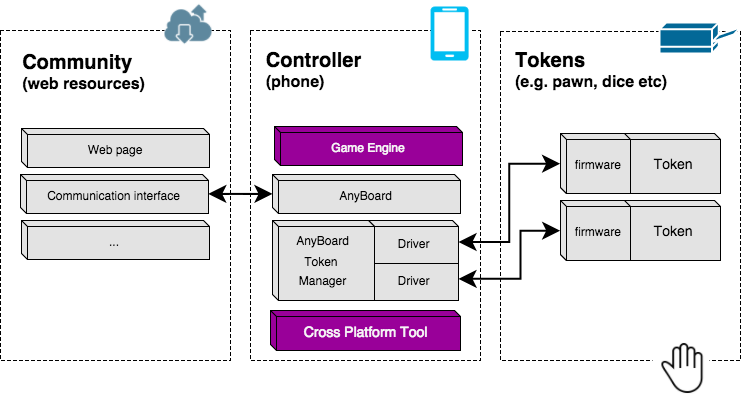
\includegraphics[width=12cm]{img/broad_architecture_idea.png}
\centering
\caption{High level components of AnyBoard.}
\label{fig:high_level_components}
\end{figure}

Game development tools and communities already exists, and hence the main part that makes the AnyBoard platform unique, is helping integrate the tangible tokens as a part of games. This is therefore the area of greatest importance. 

\emph{Standard example tokens}, with low level code implementing typical token capabilities, will be provided for developers that wish to create games with general token requirements. This token will communicate with a \emph{Token manager} on the application side that handles the communication between the game logic and physical devices. This component will provide a token API on the software side, so developers can listen to token-events and send commands without the knowledge of the low level code, as well as assist developers to create easy-to-use interfaces for connecting and initiating the game and game tokens.  \emph{(P1, D5)}

The Token manager is separated from any spesific token, and communicates through a \emph{device spesific driver}. A generic extendable driver will be provided to assist developers that wish to create their own tokens with other capabilities. \emph{(D1, D6)}

A \emph{Game engine} will provide tools that help the developer quickly create the components of his or her game. We wish to provide base components spesificly suited for hybrid board games, such as Board, Tile, Pawn, Dice etc, both the logical and visual \emph{UI} part. \emph{(D7, D8, D9)}

The AnyBoard software platform should be based on a \emph{cross platform tool} that enable games made with the AnyBoard to compile to different operating systems. \emph{(D3, D4)}

Several of these components exists already, and we aim to use open source, free-to-use, modular and well documented tools, so that a developer can pick apart the AnyBoard system and add capabilities where need be. \emph{(D1, D2)}

Lastly, a web-based home for AnyBoard can grow a community and provide information for all roles involved with hybrid board games. The AnyBoard platform could be downloaded from here, and tokens sold from a web store. It can also provide a knowledge base and tools for developers to assist each other. Through a \emph{Game Store} or an overview of hybrid board games, we hope to assist users with finding other games they can play, and an assistive IDE for game developers could help lower the knowledge barrier for new developers even further. \emph{(P2)}\footnote{A game store, or a web based IDE is a later stage than the AnyBoard platform presented in this thesis.}. 





\newpage
\chapter{Preliminary studies} \label{ch:preliminary}

\section{Cross platform tools} \label{sec:cpt}
One of the main goals of the software platform is that it should be easily accessable to use and develop on. Since we're in the early of development of the platform, the tools we choose should restrict us in the least amount of way, regarding technical capabilities. The purpose of using a cross platform tool is being able to develop for multiple platforms at once, and hence lower the development time for both us and developers making use of AnyBoard.

In order to lower barrier for new developers or other users to use the platform, AnyBoard should ideally be based on free to use tools, and written in popular languages. Code written in AnyBoard should be deployable without or with only minor modification to multiple popular platforms. Support for deploying to iOS and Android platforms is chosen as a minimum requirement, due to them covering the largest audience\footnote{According to \href{http://en.wikipedia.org/wiki/List_of_mobile_software_distribution_platforms}{http://en.wikipedia.org/wiki/List\_of\_mobile\_software\_distribution\_platforms} (Accessed 2015-05-13)}.

\subsection{Criterias}
We've judged options in regard to the following criteria:
\begin{itemize}
\item{Popularity of programming language – Projects based on languages popular in open source communities have a larger pool of potential developers to contribute to the platform}
\item{Knowledge of programming language with regards to team – The programming languages chosen should be of some familiarity to the people involved in this project }
\item{License and cost to use – Cost is a barrier for developers to contribute to the project. Like with hardware, required software should be as cheap as possible to aquire. An open source framework would be preferrable, not to create restrictions on possible functionality of the software.}
\item{Existing bluetooth capabilities - BlueTooth functionality is a requirement for the basic functionality of AnyBoard. A tool with good BlueTooth support would be preferable.}
\end{itemize}

\subsection{Candidate cross-platform tools}
The candidates were chosen from comparisons and benchmarks of cross platform tools\cite{appindex_cpt_comparison, developereconomics_cpt_comparison, thinkapps_cpt_comparison, research2guidance_cpt_benchmark2014}. Some were excluded immediately if they clearly didn't meet  our criterias, while a couple were added due to our previous experience with them.

\begin{landscape}

\begin{table}[ht]
\begin{minipage}{\textwidth} 
\begin{tabular}{llllll}
\textbf{Name}         & \textbf{Language}              & \textbf{Bluetooth}                                      & \textbf{License}                    & \textbf{Free}                                                   & \textbf{Popularity} \\


PhoneGap\footnote{\href{http://www.phonegap.com}{phonegap.com} - The original name for the Apache Cordova framework. PhoneGap is essentially Cordova with additional but optional pay-to-use services.}              & \cellcolor[HTML]{CDFBCD}JS     & \cellcolor[HTML]{CDFBCD}Yes                             & \cellcolor[HTML]{CDFBCD}Apache & \cellcolor[HTML]{CDFBCD}Yes               & \cellcolor[HTML]{CDFBCD}Very high (> 60\%) \\

Appcelerator \footnote{\href{http://www.appcelerator.com/}{appcelerator.com} – Compiles JS to native code. } & \cellcolor[HTML]{CDFBCD}JS     & \cellcolor[HTML]{FEB24C}possible (not via Appcelerator API) & \cellcolor[HTML]{CDFBCD}Apache      & \cellcolor[HTML]{CDFBCD}Yes  & \cellcolor[HTML]{CDFBCD}High (> 40\%)  \\


Cocos2d\footnote{\href{http://cocos2d.org/}{cocos2d.org} - Cross-platform game engine available in both JS, Lua and C++. Compiles to Mac OSx, Windows, Android and iOS.}               & \cellcolor[HTML]{CDFBCD}C++/JS & \cellcolor[HTML]{FEB24C}possible (not via Cocos API)    & \cellcolor[HTML]{CDFBCD}MiT         & \cellcolor[HTML]{CDFBCD}Yes                                            & \cellcolor[HTML]{FEB24C}Medium (> 20\%) \\


Unity3d\footnote{\href{http://unity3d.com}{unity3d.com} - Cross-platform framework built on an advanced game engine. Free Personal edition is limited.}               & \cellcolor[HTML]{CDFBCD}C\#/JS & \cellcolor[HTML]{FEB24C}possible (not via Unity API)    & \cellcolor[HTML]{de2d26} \textcolor{white}{Proprietary} & \cellcolor[HTML]{FEB24C}Yes*& \cellcolor[HTML]{CDFBCD}Very high (> 60\%)\\


Corona\footnote{\href{http://coronalabs.com/}{coronalabs.com} – *Limited version without access to native calls are free to use. Due to the limitations of the API and license, Bluetooth communication is unavailable for free version.}                & \cellcolor[HTML]{de2d26} \textcolor{white}{Lua}    & \cellcolor[HTML]{FEB24C}possible (not via Corona API)   & \cellcolor[HTML]{de2d26} \textcolor{white}{Proprietary} & \cellcolor[HTML]{de2d26} \textcolor{white}{Yes*}          & \cellcolor[HTML]{CDFBCD}High (> 40\%) \\


Qt\footnote{\href{http://qt.io}{qt.io}. *Free to use for open-source, non-commercial applications}                   & \cellcolor[HTML]{de2d26} \textcolor{white}{C++}    & \cellcolor[HTML]{CDFBCD}Yes                             & \cellcolor[HTML]{D8FFD7}LGPL        & \cellcolor[HTML]{D8FFD7}Yes*& \cellcolor[HTML]{CDFBCD}High (> 40\%) \\

Xamarin\footnote{\href{http://xamarin.com}{xamarin.com} – compiles C\# code to native applications. Free version has limited features.}               & \cellcolor[HTML]{CDFBCD}C\#    & \cellcolor[HTML]{FEB24C}possible (not via Xamarin API)  & \cellcolor[HTML]{de2d26} \textcolor{white}{Proprietary} & \cellcolor[HTML]{FEB24C}Yes*                    & \cellcolor[HTML]{CDFBCD}High (> 40\%) \\


Kivy\footnote{\href{http://kivy.org}{kivy.org} - Python-based framework that compiles to mobile (iOS and Android) as well as Windows, OSx and Linux. Popularity unknown, but presumed to be low compared to other alternatives.}                  & \cellcolor[HTML]{CDFBCD}Python & \cellcolor[HTML]{FEB24C}possible (not via Kivy API)     & \cellcolor[HTML]{CDFBCD}MiT         & \cellcolor[HTML]{CDFBCD}Yes                                            & Unknown \\


EvoThings\footnote{\href{http://evothings.com/}{evothings.com} - Light framework based on Cordova, with libraries centered around communication with small hardware objects (Internet of Things) and simplifying testing. Popularity unknown, but benefits from being based on Cordova. }             & \cellcolor[HTML]{CDFBCD}JS     & \cellcolor[HTML]{CDFBCD}Yes                             & \cellcolor[HTML]{CDFBCD}Apache      & \cellcolor[HTML]{CDFBCD}Yes & Unknown \\                                            

\end{tabular}
\caption {Overview over initial candidates for cross-platform compatibility. Preferable properties of the platforms are marked in light green, less preferable in orange, while undesirable properties are marked in dark red. Popularity based on developers awareness in Cross-Platform Tool Benchmarking 2014\cite{research2guidance_cpt_benchmark2014}.}
\end{minipage}
\end{table}
\end{landscape}

\subsection{Evaluation}
Cross-platform tools (CPTs) are increasing in popularity. Some of them compiles to a native application on each platform (Unity, Cocos, Appcelerator), while the others run in an "in-app browser" (PhoneGap, EvoThings), essentially acting as web pages. The latter will in most cases simplify the development and make an easier transition for existing web-developers, at the price of performance and functionality. Such tools might therefore not be an alternative for graphic-intensive games or where access to certain parts of the phones functionality. 

With the exception of EvoThings, BlueTooth capabilities is not an area of focus for any of the tools. They do however support writing own libraries or plugins or give developers the opportunity to write native code that can access bluetooth capabilities on the phone. We could also find support or plugins for PhoneGap and Qt to simplify BlueTooth access for us.

We chose three different frameworks to further investigate based on our initial findings. PhoneGap, due to it's licensing and popularity; EvoThings, for being closely related to PhoneGap and adding functionality suited for our purpose, and lastly Appcelerator Titanium for the comparison of in-browser vs native app platforms.

\subsubsection{PhoneGap}
PhoneGap by Adobe/Nitobi was the original creator of Apache Cordova, which is today the most popular engine for creating mobile cross-platform in-browser applications. The Cordova engine provides basic phone functionality such as Camera, GPS and vibration to a web based environment for creating apps. In 2011, Adobe donated the Cordova code-base to the Apache Foundation, and PhoneGap instead focused on providing services on top of the engine, such as marketing, analysis, building, support and training. PhoneGap consists today of both an Open Source fork of Apache Cordova in addition to these services. The services are optional, and most of them are pay-to-use.

\begin{itemize}
\item{+ Based on well known Cordova platform}
\item{+ No or little additional code necessary to support different platforms}
\item{- Compiles to in browser apps, giving reduced performance}
\end{itemize}


\subsubsection{EvoThings}
Evothings is a toolkit based on the Cordova platform, as PhoneGap. EvoThings is centered around the idea of "Internet of things" or "ubiquitous" computing, and it provides simplifications for communicating with several different types of tokens, as well as code examples. 

While the EvoThings toolkit itself is not very popular, valid Cordova code will be valid in EvoThings. An app developed with EvoThings could also be ported to other Cordova-based frameworks with no or only small changes in the code base. This has the added benefit of making existing Cordova/PhoneGap community relevant for development on this platform.

The additional features included in EvoThings compared to Apache Cordova is a simplification of testing by allowing instant deployment to your phone in the testing phase, using a EvoThings app. In addition, libraries to communicate using Bluetooth with external hardware is included.

\begin{itemize}
\item{+ Toolkit allows instant deployment to phones through EvoThings test suite app}
\item{+ Extra support and examples for relevant communication with external hardware through bluetooth}
\item{+ Based on well known Cordova platform, making a large existing community relevant for this platform}
\item{+ No or little additional code necessary to support different platforms}
\item{- Compiles to in browser apps, giving reduced performance}
\end{itemize}

\subsubsection{Appcelerator Titanium}
Appcelerator Titanium has a different approach than the Cordova-engine on how to create cross-platform applications. Appcelerator themselves compare Appcelerator Titanium vs PhoneGap and explain their differences. Some of their main points\footnote{According to \href{http://www.appcelerator.com/blog/2012/05/comparing-titanium-and-phonegap/}{http://www.appcelerator.com/blog/2012/05/comparing-titanium-and-phonegap/} - "Comparing Titanium and PhoneGap" (May, 2012)} is that:

\emph{The barrier to entry in using PhoneGap to package web pages as native apps is extremely low.} - Starting developing with PhoneGap requires very little knowledge or experience with creating mobile applications, or knowing the difference between platforms. Knowledge of creating web applications is sufficient for starting to create PhoneGap applications for different platforms.

\emph{Very few native APIs are exposed to PhoneGap applications by default} - While PhoneGap by default only provides functionality that are common among different phones, Titanium has a richer set of functionality available from the phone. A Titanium-based app can be better tailored to fit and use all of the capabilities of a phone.

\emph{The quality of the user interface in a PhoneGap application will vary based on the quality of the web view and rendering engine on the platform.} - Since the user interface of PhoneGap is based on an in-browser app, it will not look like a native app with native controls and buttons. The performance of a browser interface will also be slower than interfaces made up of the phones native controls. In addition, due to browser differences, the interface might look different between platforms. 

\emph{The scope of the Titanium API makes the addition of new platforms difficult – implementing the Titanium API on a new native platform is a massive undertaking}. The price to pay for being able to create tailored apps for each platform is a lower code re-usage. Considerably more time must be spent for porting an application from one platform to another. 

\begin{itemize}
\item{+ Compiles to native code, providing better performance than in-browser apps}
\item{+ Can be better tailored by use of native UI of each OS.}
\item{+ Provides a richer set of phone functionality}
\item{+ Has optional pay-to-use platforms}
\item{- Higher barrier for new developers}
\item{- Lower code re-usage (60-90\%) than in-browser-apps, requiring effort to port app to different platforms}
\end{itemize}

\subsection{Conclusion}
From our findings we interpret that the Cordova-platform has a lower barrier for entry than Titanium. We believe that the performance advantage, and access to native UI of Titanium in our case is of less importance than keeping this barrier to a minimum, and holding code re-usage to a maximum. This is large part due to our low need for a high performance app, and our requirement of low barrier to contribute to the platform \ref{sec:high_level_requirements}.

Between PhoneGap and EvoThings, the difference seems to be small due to them both being based on a Cordova engine. Applications made in EvoThings are designed to be built as Cordova apps\footnote{As shown in \href{http://evothings.com/doc/build/cordova-guide.html}{http://evothings.com/doc/build/cordova-guide.html}}, which are compatible with PhoneGap. Therefore, we have chosen to develop and test in the EvoThings framework. Its suitability in our project with regards to Bluetooth devices and communication with tangible hardware is unmatched. It also provides a few very handy development features, such as instantaneous deployment to the phone. This allows for rapid testing and development .
If the services PhoneGap provides is of interest later, a transition to using that is expected to go swiftly.




\section{Game engines}
The purpose of a game engine (GE) is to structure the game components and allow reuse of its code in different games. It also provides features for common components of games, such as file loading, audio playing and graphics handling among other things. In large part, the AnyBoard platform is a GE for hybrid board games, albeit a simple one. It also differs in that AnyBoard provides board game entities, and communication with tangible devices. This is unlike typical GEs, that rather focus on timing, sound and graphics. Since creating a GE is a massive task, we would like  to reuse existing open source game engines to include these features in AnyBoard or find game engines that can complement the functionality of AnyBoard when used side by side.

Common features of a GE include:
\begin{enumerate}
\item \textbf{Graphics engine/Renderer} – assisting the rendering of graphical elements on the screen. 
\item \textbf{Map creation tools} - providing an easy way to create maps (or in our case boards), and structures suited for abstracting locations and its properties.
\item \textbf{Asset handler} - Early loading of game assets can put unnesessary load on memory, while late loading can lead to a low performance. An asset handler loads the game elements at an appropriate time. 
\item \textbf{Physics Engine and collision detection} - giving the game a realistic feeling of physics. 
\item \textbf{Artificial Intelligence} - Some game engines provide components to support creating computer-based opponents.
\item \textbf{Signals and event handler} - With the exception of certain genres, games are commonly based on events intiated by the player, such as clicking buttons or interacting with elements in the game. A game engine often includes mechanisms that helps notify parts of the system that have registered to such events.
\item \textbf{Other} - Game engines can also provide simplification for networking in order to support multiplayer games or interactions with internet servers.
\end{enumerate}

The purpose of finding a suitable GE is to enable the development of more complex games in collaboration with AnyBoard. When using an established GE, one can create game with complex graphics, scale graphics, create maps or play sounds more easily than without. If examples of AnyBoard is displayed in collaboration with popular GEs, we might also be able to more quickly recruit developers from that community. 
\subsection{Criteria}

We've judged our options for a GE in regards to the following criteria:
\begin{itemize}
\item Licensing - As with other parts of the software platform, we prefer an open source, free-to-use game engine.
\item Compatibility – As we have chosen EvoThings (Cordova-based) as cross platform tool, a game engine based on the same programming language (JavaScript) would there be preferable. 
\item Popularity and activity - We want the software platform to be based on tools that are popular and are being actively developed. We've judged this on 1) Number of developers that have marked the repository as a favorite. 2) Number of code-changes done to the repository the last 12 months
\item Performance - As one of the drawbacks of Cordova is performance, we wish for the game engine to be as light and efficient as possible. This can be hard to judge without testing, so we have used library size as a proximity to this. We have also looked at whether or not mobile platforms seems to be a target audience for the platform.
\end{itemize}

\subsection{Candidate game engines}
There is a large community around JavaScript, and there are a lot of options for a JavaScript-based game engine. Our candidates has been chosen from overview and comparisons by several community resources such as HTML5GameEngine\footnote{\href{https://html5gameengine.com/}{html5gameengine.com}} and Github\footnote{\href{https://github.com/showcases/javascript-game-engines}{github.com/showcases/javascript-game-engines}}. Several were excluded immediately if they clearly didn't meet our criteria.

\begin{table}[ht]
\begin{minipage}{\textwidth} 
\begin{tabular}{llllll}
{\bf Framework} & {\bf License} & {\bf Size\footnote{Size of minified JS libraries. Libraries marked with * are unminified size (minified should be about 60 percent smaller)}} & {\bf Activity\footnote{Files changed/additions/deletions in the 12 months between June 2014 to June 2015. k = thousand}} & {\bf Community\footnote{Number of favorites/Number of contributers to repository pr. June 2015}} \\
CraftyJS& \cellcolor[HTML]{CDFBCD}MiT & 99KB & \cellcolor[HTML]{CDFBCD}81/7k/3k   & \cellcolor[HTML]{CDFBCD}1772/97 \\
LimeJS & \cellcolor[HTML]{CDFBCD}Apache & 200KB* & \cellcolor[HTML]{de2d26} \textcolor{white}{5/54/21}  & \cellcolor[HTML]{CDFBCD}1320/30 \\
ImpactJS& \cellcolor[HTML]{de2d26} \textcolor{white}{Propr.} & & & \\
Ludei   & \cellcolor[HTML]{de2d26} \textcolor{white}{Propr.} & & & \\
EnchantJS & \cellcolor[HTML]{CDFBCD}MiT & 225KB* & \cellcolor[HTML]{de2d26} \textcolor{white}{19/202/282} & \cellcolor[HTML]{CDFBCD}1300/25 \\
MelonJS & \cellcolor[HTML]{CDFBCD}MiT & 168KB & \cellcolor[HTML]{CDFBCD}333/14k/8k & \cellcolor[HTML]{CDFBCD}1367/33 \\
Quintus & \cellcolor[HTML]{CDFBCD}MiT  & 20KB& \cellcolor[HTML]{FEB24C}17/793/509 & \cellcolor[HTML]{CDFBCD}1000/29 \\
Phaser & \cellcolor[HTML]{CDFBCD}MiT  & 692KB& \cellcolor[HTML]{CDFBCD}1.1k/230k/117k & \cellcolor[HTML]{CDFBCD}8694/140 \\

\end{tabular}
\caption {Overview over candidates for game-engine. Preferable properties of the platforms are marked in light green, less preferable in orange, while undesirable properties are marked in dark red.}
\end{minipage}
\end{table}
\subsection{Evaluation}
We have chosen CraftyJS, Phaser and Quintus to evaluate further. 

All of these have compatibility with with Tiled\footnote{Tiled (\href{http://mapeditor.org}{mapeditor.org}) - an commonly used editor for creating game maps.} - a visual game map editor for creating maps. All three also support our other basic technical requirements, such as signal/event handlers, and have examples that indicate performance beyond our requirements.

\textbf{Quintus} is some way just what we want. It's a simple library that covers our basic technical requirements, and seems to support extendability well. It was originally made as an example for a book on game development, HTML5 Game Development\cite{rettig2012professional}, and is therefore well documented. They say on their own website\footnote{\href{http://www.html5quintus.com/guide/core.md}{html5quintus.com/guide/core.md}} that it \emph{does very little game-wise by itself and provides little more than a backbone for the other modules to build around}.

Its downside is a low level of activity and small community. Its lower amount of activity can to some extent be contributed to lower code base size, but the difference in community from Crafty and Phaser still shows that Quintus is not as well established and polished. On their Github page\footnote{\href{https://github.com/cykod/Quintus}{github.com/cykod/Quintus}} it states \emph{"Warning: Quintus is at a very early stage of development, use at your own risk.*"}.

\textbf{CraftyJS} is a larger library than Quintus, and provides a richer set of built in functionality. Documentation seems to leave us with the impressions of a modular and easily extendable architecture. One comparison of Phaser and Crafty\cite{phaser_vs_craftyjs} has listed this as the main advantage of Crafty. It supports mobile, even though that's not a focus from the looks of their webpage.

\textbf{Phaser} is clearly the most mature and popular of the alternatives we have investigated. Phaser have more game examples and thorough guides than our other candidates. The framework has support for TypeScript and JavaScript in addition to providing an in-browser game editor. Its graphics engine is PixiJS, a standalone webGL renderer which claims performance to be their strength. 

Phaser seems suited for this project in many ways. It's focus is mobile, and provides a scaling manager component for handling various screen sizes. It has the community and guides to make it easily understood and learnt, and feels like a solid component to base our project upon.

Our only concern is the suitability for such a polished product to be integrated in AnyBoard. While it does provide a plugin system, it could be difficult to encapsulate Phaser in a new framework. Users have reported that Phaser can feel clumsy and not modular enough\cite{phaser_vs_craftyjs, search_for_javascript_ge}, which can make it hard to break apart and reuse relevant parts alone.

\subsection{Conclusion}
Both Quintus, Crafty and Phaser covers our basic criteria. Their differences lies mainly in size, amount of functionality and popularity. The more popular, the more solid it seems, and the less functionality will we be required to make from scratch. On the other hand, it can be harder to encapsulate and reuse only parts of the GE, and the game engine part end up being unnecessary heavy.

In other words, Quinitus is a great choice for learning purposes, and accompanied by its book\cite{rettig2012professional} developers could learn about game engines, HTML5 game development, and then reuse that knowledge and parts or whole of Quintius in collaboration with AnyBoard.

Phaser on the other hand, seems to have a great community behind it, and has an appealing mobile-first focus. We believe creating examples with Phaser could spark interest among its large community and existing developers. This GE could also be used in collaboration with AnyBoard simplify the making of professional and polished games. However, its size and complexity might prove too difficult to dissect and integrate with AnyBoard.

Due to these observations, and the very dynamic and active environment around game development in JavaScript, we will attempt to create AnyBoard as a \emph{standalone} platform, independent of other GEs. This will allow developers to use their own preferred library in collaboration with AnyBoard. \emph{When providing examples where a GE is needed, we will go for Phaser} due to it having the largest community.


\newpage

\chapter{System Design}

\section{Requirement spesification} \label{sec:requirements}
The requirements are written as stories inspired from agile methodologies. Instead of attempting to write a complete and detailed description of the system, where all requirements is to be implemented, we have written down a backlog of conceivable requirements and wishes, and implemented them with what we assert to be the most important ones first. Requirements are subject to change, and some have not been implemented either due to time or proving unnecessary during the development phase.

\subsection{Non-functional requirements}
Considering that our goal is for the AnyBoard library to be used by different developers for creating games, as well as further developed and maintained, we wish to lower the threshold and difficulty of using the library, as well as contributing to it.

We believe this is done by creating the library and environment in the following ways:

\textbf{NFR-1, Setup should be simple, for both game developers and developers of AnyBoard} - The first barrier of development is setup of the environment. To minimize this, a developer should ideally have to go through as few as possible steps before he or she can use the library, or contribute to it. This is relevant both to the game developer using AnyBoard as a library to create their own game, as well as a developer that wish to contribute or change the AnyBoard library itself.

We believe a simple setup is important for curious developers to test the library, and for more dedicated developers to take the step and modify it for their own needs.

\textbf{NFR-2, AnyBoard should be provided with a rich set of examples} - A common way of understanding the usefulness and workings of any programming library is looking at simple examples demonstrating the code syntax, function and the effects of using that library. They can work both as a way of marketing the library to game developers, and a way of assisting developers in need of help or a starting point for their own game.

This can be done through publishing the code of complete games built with AnyBoard platform, as well as through small code snippets demonstrating some concrete functionality or even test code.

We believe examples are very important for the adoptation of the AnyBoard library by game developers.

\textbf{NFR-3, The features and functionality of AnyBoard should be tested, and easily available} - Tests should be implemented, so that one can confidently change parts of the code without unknowingly breaking part of the code, as well as providing small examples of library usage.

As a code-base grows in size, the barrier to contribute to the code base increases. There are more classes and functions to be understood before one feels confident. One can often feel uncertain of how changing one part of the code affects the rest of the code base, and in fear of breaking some other functionality unknowingly, refrain from changing anything. 

Having written tests for the functionality of the software, can dramatically lower the fear of unknowingly breaking parts of the code-base, and as such lower the barrier for contributing to the AnyBoard library. It also provides examples of how features are used and expected to work, which complements rich examples as well as documentation.

We believe tests are very important for the further development of the AnyBoard library.

\textbf{NFR-4, AnyBoard must be consistently documented, in an accessible and understandable matter, both for new and experienced developers} - Non-internal elements of the framework (Classes and methods intended to be public) should be well documented. Names, parameters and types of parameters should be easily attainable. 

The larger a code base is, the more complex and harder to understand it usually becomes. By providing good documentation, in form of both in-line coding, auto-complete functionality for editors and online documentation, we lower the time used by both game developers and developers of the library to understand and use the it. 
We believe that providing good documentation is vital for the chances for the library to be used and developed further.

\textbf{NFR-5, AnyBoard should strive to have decoupled code, as to maximize re-usability of different parts, and be independent of other libraries} - Code should be decoupled, so parts can easily be replaced without having cascading effects on other parts of the code base. 

An example of this would be using dependency injection: The token manager for instance will be using some sort of bluetooth communicating capabilities in order to communicate with the token. By passing the bluetooth driver to the AnyBoard TokenManager class upon creation, instead of directly calling the bluetooth drivers we know of, the bluetooth communication libraries will be decoupled from the AnyBoard library. 

Decoupling of code allows changing or replacing parts and dependencies of the our library more easily. 

\subsection{Functional requirements}


\begin{table}
\centering
\caption{Functional requirements for token capabilities}
\label{freq:token}

\begin{tabular}{ | m{1cm} | m{9cm}| m{1.5cm} | }
     & {\bf Functionality}                                                                                                                                                                                                                                                       & {\bf Priority} \\
FT-1 & \emph{As a developer}, I need a token manager that holds all tokens, so I easily can obtain the individual tokens instances from different parts of the code.                                                                                                                    & Low            \\
FT-2 & \emph{As a developer}, I want the token manager to be able to scan for and return active tokens nearby, so I'm not required to have intimate bluetooth knowledge.                                                                                                                & High           \\
FT-3 & \emph{As a developer}, I want to be able to replace the token driver without changing my game code, so I can efficiently test and try different tokens.                                                                                                                          & High           \\
FT-4 & \emph{As a developer}, I want tokens to trigger events upon token-token events or token-constrain events, and allow me to subscribe to this and other events, so I can respond to token interaction. & High         \\
FT-5 & \emph{As a developer}, I want to be able to obtain standard tokens and drivers, so I can quickly create a game without having intimate knowledge of hardware or low-level code.      & High           \\
FT-6 & \emph{As a developer}, I need to be able to test how my game is using tokens and responding to token interactions within a digital interface, and not have to use physical tokens for testing, so I can test more efficiently and develop games with tokens I have not acquired. & Medium \\

FT-7 & \emph{As a developer}, I need to be able to connect simultaiously to at least 4 different tokens. & High 
\end{tabular}
\end{table}

\begin{table}
\centering
\caption{Requirements for graphical interface entities}
\label{freq:graphic}
\begin{tabular}{ | m{1cm} | m{9cm}| m{1.5cm} | }
     & {\bf Functionality}                                                                                                                                                                                                          & {\bf Priority} \\
FG-1 & \emph{As a developer}, I want to be able to create menus and menu items that link to new screens or internet web, so I can create a menu-feature quickly                                                                            & Low            \\
FG-2 & \emph{As a developer}, I want to be able to quickly be able to create a rule-screen from a set of written rules and a FAQ from a set of questions, so I can create this feature quickly. & Low            \\
FG-3 & \emph{As a developer}, I wish to be able to retrieve rules and FAQ from a web page, so I don't have to have duplicate information in case I have a web page.                       & Low           
\end{tabular}
\end{table}

\begin{table}
\centering
\caption{Functional requirements for game entities}
\label{freq:game_entities}
\begin{tabular}{ | m{1cm} | m{9cm}| m{1.5cm} | }
     & {\bf Functionality}                                                                                                                                                                                                                                                                                                     & {\bf Priority} \\
FE-1 & \emph{As a developer}, I want to be able to build on a generic Resource model, so I don't have to spend time implementing interactions such as paying, trading or giving resources between Players and/or the Game.                                                                 & High           \\
FE-2 & \emph{As a developer}, I want to be able to build on a generic Card and Deck model, so I don't have to implement standard usages such as shuffling, drawing, playing.                                                                                                                                                          & High           \\
FE-3 & \emph{As a developer}, I want to be able to build on a generic Player model, that holds a Pawn, has a set of resources, a set of cards, a set of missions, points and  similar, so I don't have to implement those & High           \\
FE-4 & \emph{As a developer}, I want to be able to build on a generic Dice model, so I don't have to spend time implementing interactions such as rolling and returning values from a set of dices. & High           \\
FE-5 & \emph{As a developer}, I want to be able to build on a generic Timer model, so I can create events that happens at a set amount time into the game, or after an event.                                                                                                                                                         & Low            \\
FE-6 & \emph{As a developer}, I want to be able to build on a generic Turn model, so I can quickly specify what goes into each turn of a player.                                                                                                                                                                                      & Medium         \\
FE-7 & \emph{As a developer}, I want to be able to build on a generic Board and Tile model with listeners and triggers, so I can quickly specify where one can go from which tile, their distance, what happens when one steps on a tile without having to create the models from scratch. & High           \\
FE-8 & \emph{As a developer}, I want to be able to log events of different severity, and be able to see them, so I can debug my code and see where something fails                                                                                                                                                                    & High           \\
FE-9 & \emph{As a developer}, I want to be able to assign properties and fields to all my models, so I can create my own concepts and define my own properties on top of the existing models. & High
\end{tabular}
\end{table}

Here we present stories that relate to the hardware tokens and the interaction between those and the software platform.

\subsubsection{Tokens}
The ability for simple interaction with tokens is the main feature of AnyBoard that sets it apart from other game engines. Hence, the requirements relating to this is the main part of the platform. Our requirements are shown in table \ref{freq:token}, and is related to simple scanning, connecting and listening to tokens and its interactions as well as decoupling tokens from game code.

\subsubsection{Graphics}
Board games will include common features, such as menus or rules for games. We wish to provide common entities for quick development of these graphical elements. The requirements relating to this are shown in table \ref{freq:graphic}. 

\subsubsection{Entities}
Table \ref{freq:game_entities} shows the requirements relating to logical board game entities. Hybrid board games will include many of the same entities, which was described in section \ref{sec:boardgames_commonalities}. We believe it could be useful for developers to have these available.

\newpage
\section{Application architecture}
AnyBoard will exist over 3 types main parts, as first shown in figure \ref{fig:high_level_components}. \textbf{Tokens}, such as the AnyBoard pawn, or printer, are the tangible pieces that users can interact with. Tokens talk with the second part, the \textbf{Controller}. The controller is run on a smart device, such as a mobile phone or a tablet. Here, all the logic lies for the game, including the rendering of graphics. The third part is a web based community. This part is conceptual, and will not be implemented in this thesis. The application architecture that we will work on in this thesis, consists therefore of the controller and token part, which is shown in figure \ref{fig:overview_architecture}. 
\begin{figure}[ht]
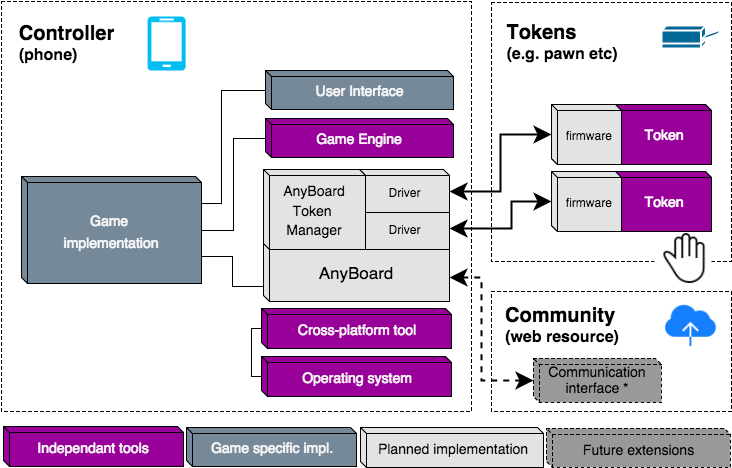
\includegraphics[width=12cm]{img/overview_architecture}
\centering
\caption{Architecture overview. AnyBoard will exist over three components. Tangible tokens such as digital pawns, a game controller/hub running on a smartphone, and an online application assisting the a community of both developers and players. My contribution in this thesis consists of the light grey boxes, denoted "Planned implementation".}
\label{fig:overview_architecture}
\end{figure}

\section{Phone-Token communication}
The means of communicating easily with different tokens is the most central component of AnyBoard. We aim for decoupled token-specific code, to address the requirements in table \ref{freq:token}.

TokenManager is a static component that handles the scanning and connecting/disconnect to tokens.
Its purpose is to identify nearby tokens, and determine an appropriate driver for the token to use. TokenManager has an own driver for this purpose. 

In figure \ref{fig:anypawn_architecture} we see this illustrated. Upon finding suitable drivers for detected tokens, TokenManager instantiates Token A1, Token A2 and Token B. These are Token Class instances, which – seen from the developers point of view – work as a sort of API on top of the tokens. These abstract away the low level communication and commands between AnyBoard and the specific tokens, and provide affordances such as ledOn(), ledOf() and print() functions.

\begin{figure}[ht]
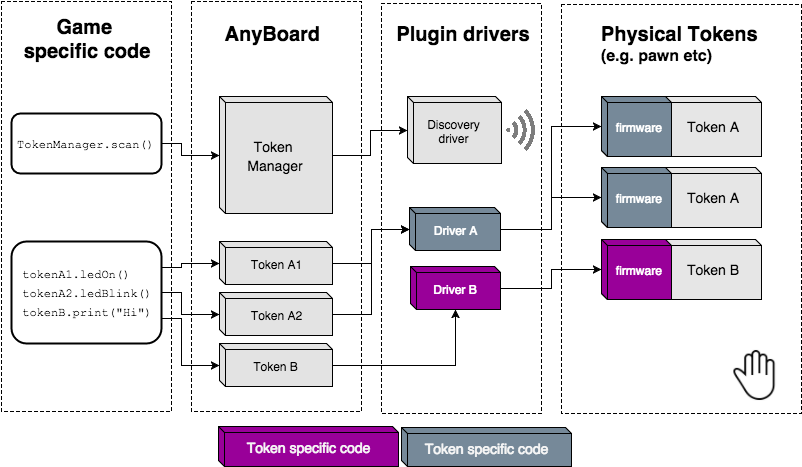
\includegraphics[width=12cm]{img/design_tokenmanager}
\centering
\caption{Communication overview between phone and token. An example where three tokens are discovered by the discovery driver and mapped to two different drivers, which handles the communication with their compatible tokens.}
\label{fig:anypawn_architecture}
\end{figure}


\section{Web-Phone communication}
Web is a component of AnyBoard that will not be implemented in this project, and will hence not be discussed or designed in any detail here. However, it's worth to note some thoughts about this important capability.

We imagine to use HTTP-communication where the phone sends requests to a API on the server. Suggested uses for this communication are:
\begin{enumerate}
\item Retrieving updated FAQ for the game.
\item Sending of events and actions in the game to enable multiplayer functionality, or viewers to watch a game.
\item Sending of events and actions in the game for history/logging.
\item Gathering statistics of usage.
\item Download new games from a Game store
\item Retrieve updates for a current games
\end{enumerate}

The basic tool necessary to enable this sort of communication is capability of communication over the HTTP-protocol. This capability could also be a useful feature for developers that wish to encapsulate web services into their board game or use physical devices that communicate using web APIs. 

This capability is already built into the JavaScript language, with the class XMLRequest. Abstracted HTTP calls using Ajax is also available in a variety of other JavaScript libraries. We therefore see no obstacles for this capability, even without designing for it in the current phase.
\newpage
\chapter{System implementation} \label{ch:implementation}

This chapter describes the implementation of AnyBoard library. We follow the chronological implementation of the library, by starting with the setup of the environment, then the entities of the board game, followed by bluetooth communication and token implementation. We'll describe what technical choices were made, our motivation for them, and what part they play in the project. 

\section{Development environment}
During the development of AnyBoard, we have used some tools to simplify certain tasks for us. This section explains the different elements and tools that we have used during development of the AnyBoard library. These tools are not required, nor related to the use of the AnyBoard framework in creating board games, only in the development of the library itself. All of these tools can also be discarded and/or replaced without having any effect on the functionality of the AnyBoard platform.

For the implementation of the AnyBoard platform itself, see section \ref{impl:entities}

All tools used here are based upon a NodeJS platform. Developing AnyBoard in this environment is therefore supported by those operating systems that support NodeJS (Linux, Mac OSX, Windows, SunOS). 

\begin{figure}[ht]
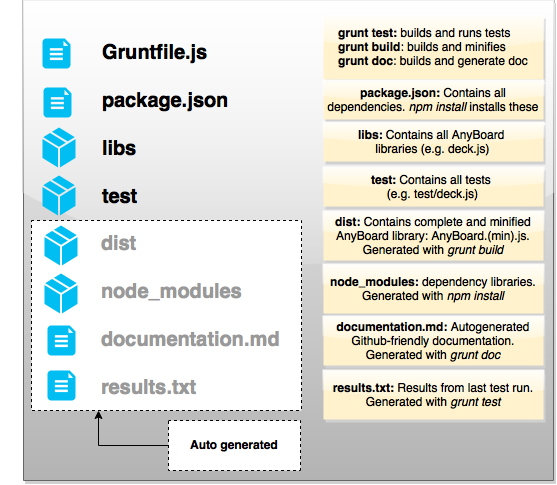
\includegraphics[width=12cm]{img/anyboard-development-overview}
\centering
\caption{Overview over the AnyBoard development files and folder structure.}
\label{fig:anyboard_development_overview}
\end{figure}

\subsection{Platform and dependency handler: NodeJS}
NodeJS\footnote{\href{http://nodejs.org}{nodejs.org}} is a platform built on Chrome's JavaScript runtime for easily building fast, scalable network applications. It is used in the project as a dependency handler and platform for our other tools, i.e. it gives us the opportunity to use the other . 

\subsubsection{Motivation}
We have chosen to use NodeJS as a tool in this project due to the active community around it, which has resulted in it being a reliable platform with a rich variety of tools that can be found and used with it. In this project, it provides us with a large set of possible tools and libraries to simplify development. It also gathers all dependencies and specifies them in one file, and provides a \emph{\textbf{simple setup}} of dependencies for the environment. 

Being the by far most dominent JavaScript-based platform and something that we have previous experience with, we have not considered other options.

\subsubsection{Usage}
In figure \ref{fig:anyboard_development_overview} \emph{package.json} is a node package file for AnyBoard. It gives meta data about AnyBoard, such as location of online repository and version number, in addition to specifying all dependencies that should be installed in order to set up the development environment. Installing all dependencies is as easy as installing NodeJS, followed by navigation to the folder in a terminal and typing \emph{npm install}.

Upon installing dependencies, those are automatically installed under the \emph{node\_modules} folder, shown in the auto generated section of figure \ref{fig:anyboard_development_overview}.

\subsubsection{Replacing NodeJS}
Not using or replacing NodeJS will require changing most of the development environment, including test framework and task runner, but has no effect on the functionality of the AnyBoard library.

\subsection{Test framework: MochaJS}
Mocha \footnote{\href{http://mochajs.org/}{mochajs.org}} is a JavaScript-based test framework. It is used in the project in providing an easy to understand syntax in writiting tests, and reports the results of tests in a readable manner (see figure \ref{fig:mocha_result}). 

\subsubsection{Motivation}
Testing frameworks provides a clear syntax for testing, as well as methods and constructs for asserting whether or not function work as intended. Using a test framework and \emph{\textbf{writing tests}} for our library provides confidence to developers that they don't break the code unknowingly when changing the code. It also \emph{\textbf{provides examples}} of how to use the library.

We have chosen MochaJS over alternatives like UnitJS\emph{\href{http://unitjs.com/}{unitjs.com}} and VowsJS due to our familiarity with it, and great reporting format.

\subsubsection{Usage}
Our tests are located within the \emph{test} library shown in figure \ref{fig:anyboard_development_overview}. They are named with the same name as the library in the \emph{libs} folder that they test. All .js files placed in this folder will automatically be run by our MochaJS installation upon running \emph{grunt test} from the console when located in this folder.

\subsubsection{Replacing MochaJS}
Changing the choice of test framework will require rewriting at least parts of the tests, but has no effect on the functionality or build of the AnyBoard library, nor documentation.

\begin{figure}[ht]
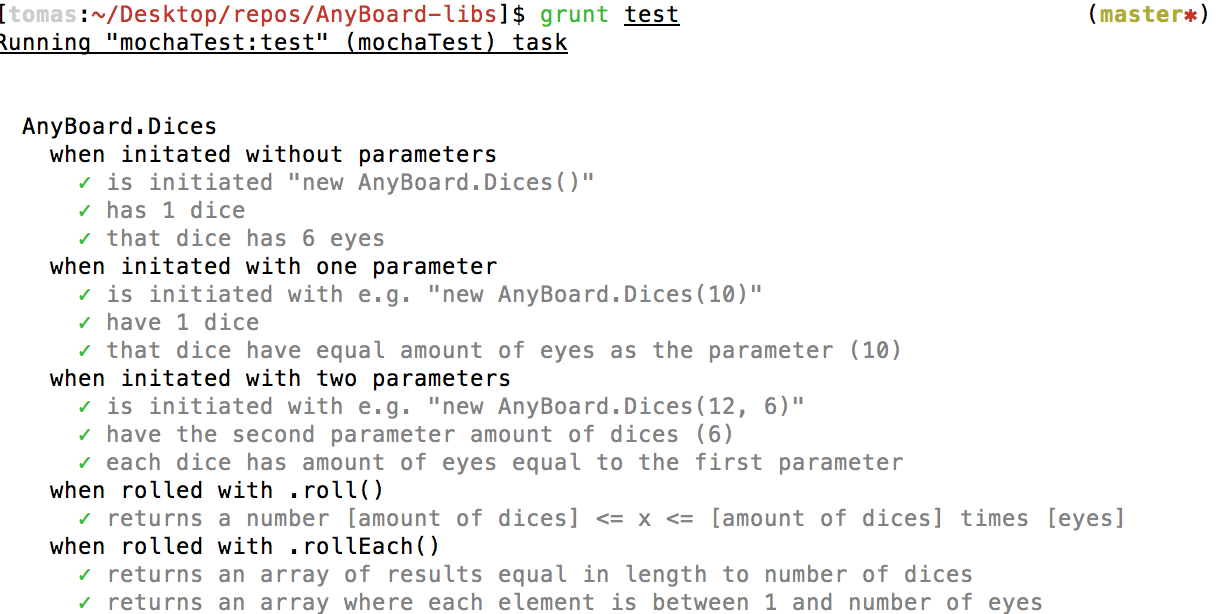
\includegraphics[width=12cm]{img/mocha-result}
\centering
\caption{Human readable test results from unit tests made with Mocha test framework.}
\label{fig:mocha_result}
\end{figure}

\subsection{Task runner: Grunt}
Grunt\footnote{\href{http://gruntjs.com/}{gruntjs.com}} is a JavaScript-based Task Runner. It is used in the project to simplify building the AnyBoard library, generating documentation and running tests.

\subsubsection{Motivation}
Task runners simplify common tasks, such as concatination of files, compilations etc. by allowing us to create shorthand commands for doing larger tasks. Our motivation is simplifying the creating of documentation files, concatination and minifying our library from smaller modules. 

Grunt was chosen over alternatives such as GulpJS\footnote{\href{http://gulpjs.com/}{gulpjs.com}} and BroccoliJS\footnote{\href{http://broccolijs.com/}{broccolijs.com}} due to our prior experience with it, as well as larger community.

\subsubsection{Usage}
\emph{Gruntfile.js} as shown on top in figure \ref{fig:anyboard_development_overview}. The file specifies 7 different tasks, that is run by \emph{grunt "taskName"}, where the different "taskName" are specified in bold below. The first four tasks are simple tasks that have names dictated by a corresponding grunt module, whereas the last three are combinded tasks of which we have selected the name.

\begin{itemize}
\item \textbf{concat} - concatinates all javascript files located in \emph{lib} folder into one file, that is then put into \emph{dist/AnyBoard.js}.
\item \textbf{uglify} - Takes \emph{dist/AnyBoard.js} and compresses/minifies it, and stores it in \emph{dist/AnyBoard.min.js}
\item \textbf{mochaTest} - runs all javascript files located in the \emph{test} folder, and report their successes to the console. The result is also (over-) written to \emph{results.txt}
\item \textbf{jsdoc2md} - reads through \emph{dist/AnyBoard.js} and interprets the commenting. A markdown-file is generated and (over-) written to \emph{documentation.md}
\item \textbf{build} - runs \emph{concat} followed by \emph{uglify}
\item \textbf{test} - runs \emph{build} followed by \emph{mochaTest}
\item \textbf{doc} - runs \emph{build} followed by \emph{jsdoc2md}
\end{itemize}

\subsubsection{Replacing Grunt}
Replacing Grunt with Gulp, Broccoli or another task runner will involve replacing grunt modules specified in \emph{package.json} with modules designed for the new task runner, as well as replacing the \emph{Gruntfile.js} file with a new configuration file. It has no effect on the functionality of the AnyBoard library.

\subsection{Documentation generation: JSDoc and grunt-jsdoc-to-markdown}
JSDoc\footnote{\href{http://usejsdoc.org/}{usejsdoc.org} - a JavaScript documentation syntax and parser} is a standardized way of documenting JavaScript code. It allows IDEs\footnote{IDE is shorthand for Integrated Development Environment and is simply put a rich featured editor.} to give assisting information to a developer about the code he's using, which classes and methods are available, what they return, take as parameters etc. 

In addition, software plugins for our development platform (NodeJS + Grunt) exist that allows us to generate automatic documentation based on JSDoc syntax.

\subsubsection{Motivation}
Documenting code usually makes the further development and maintainance of code simpler. Doing it in certain ways, will also allow developers that create games with the AnyBoard libraries to be informed of which AnyBoard classes and methods that are available in his environment, as well as providing parameter list and types, provided they use a compatible IDE.

A third reason is the automatic generation of human readable documentation files, such as HTML or MarkDown files, that can be used to inform new developers of their available tools in the AnyBoard platform. Generating this documentation automatically instead of writing it manually saves us time, and gives us \emph{\textbf{consistency between different sources of documentation}}, namely from the IDE, inline code and online documentation.

We have chosen to document our code with JSDoc-oriented syntax over YUIDoc and Doxx due to JSDoc doing source parsing\footnote{JSDoc consideres source code in addition to comments in order to generate documentation}, and high extensability. 

For the plugin that runs the documentation generation, we have used grunt-jsdoc-to-markdown\footnote{\href{https://www.npmjs.com/package/grunt-jsdoc-to-markdown}{grunt-jsdoc-to-markdown} - a grunt package generating Github friendly documentation generator of JavaScript files commented with JSDoc syntax, that we decided to use}), over jsdox\footnote{\href{https://www.npmjs.com/package/grunt-jsdox}{grunt-jsdox} - a another documentation generator of Javascript files using JSDoc syntax} due to its very readable output designed for Github pages (which the project already uses).

\begin{figure}[ht]
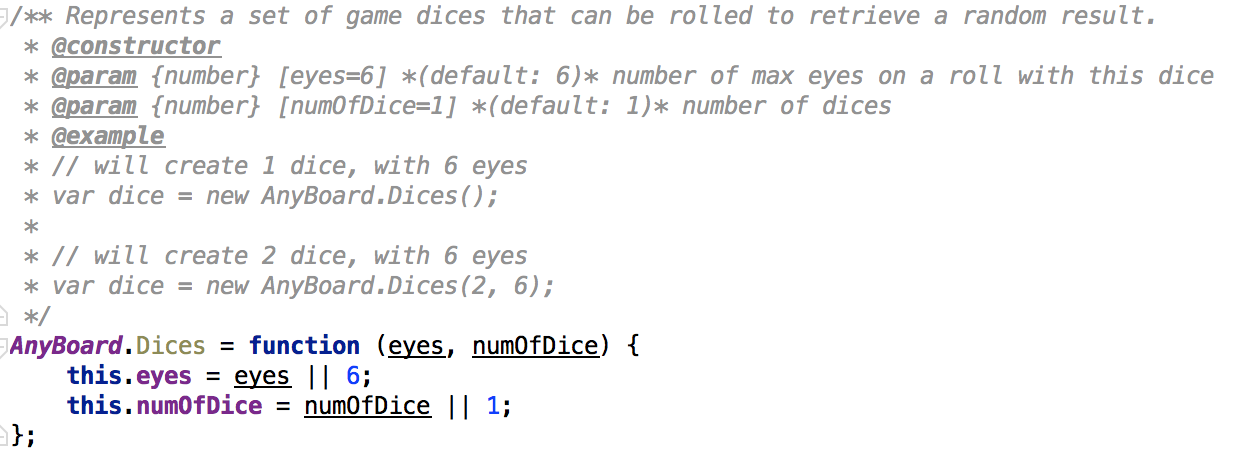
\includegraphics[width=12cm]{img/jsdoc-example}
\centering
\caption{Example of jsdoc commenting in source code.}
\label{fig:jsdoc_example}
\end{figure}

\begin{figure}[ht]
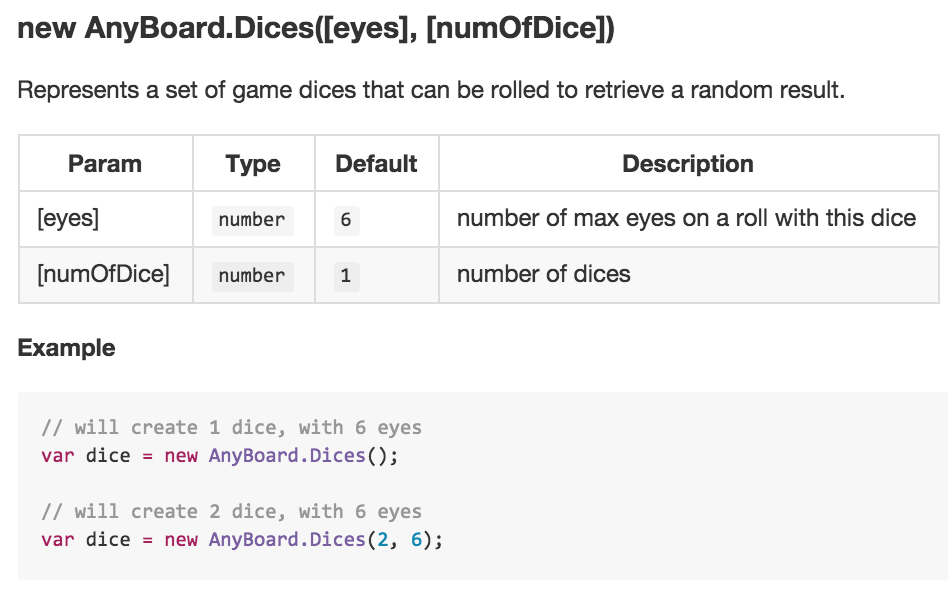
\includegraphics[width=12cm]{img/jsdoc-result}
\centering
\caption{Example of generated documentation by grunt-jsdoc-to-markdown.}
\label{fig:jsdoc_result}
\end{figure}

\subsubsection{Usage}
All source files are commented with JSDoc-syntax, see figure \ref{fig:jsdoc_example}. Most IDEs and some regular editors will automatically pick up on these comments and assist developers with writing code.

Our grunt command \emph{grunt doc}, autogenerates the \emph{documentation.md} documentation file, see \ref{fig:jsdoc_result}

\subsubsection{Replacing JSDoc}
Minor changes would be required to all source file comments in order to change to a different syntax for commenting. In addition, one would naturally have to replace grunt-jsdoc-to-markdown.

\subsubsection{Replacing grunt-jsdoc-to-markdown}
Replacing grunt-jsdoc-to-markdown will require finding a suitable grunt-compatible jsdoc compatible documentation generator, and replacing \emph{grunt-jsdoc-to-markdown} in the \emph{package.json} file.

\section{AnyBoard entities} \label{impl:entities}

\subsection{Players} 


\subsection{Decks of cards}


\subsection{Resources and transactions}

\subsection{Dice}

\subsection{Summary}


\section{Phone-Token communication} \label{impl:ble_communication}
Tokens are the physical objects for players to interact with during the game play, such as a pawns or dices. The previous work with the Don't Panic game was done using Sifteo cubes\footnote{Sifteo cubes, a commercial hardware piece that was originally used for Don't Panic \href{https://en.wikipedia.org/wiki/Sifteo\_cubes}{https://en.wikipedia.org/wiki/Sifteo\_cubes}}, a commercial device that could be adapted to work with Don't Panic using Bluetooth communication. Sifteo cubes are no longer aquireable and the lack of alternatives has led to prototyping at NTNU of a new Arduino-based token by Simone Mora. This thesis has been written with Simone as co-supervisor, and the AnyBoard framework has therefore been tested with and constructed with that token spesifically in mind, which we will from now on address as AnyBoard Pawn. 

We have also tested with a commercially available general purpose Arduino-based chip, The Lightblue Bean\footnote{The LightBlue bean (\href{http://punchthrough.com/bean/}{punchthrough.com/bean}) is a small commercially available Ardunio-based chip with built in LED, accelerometer and thermometer}.

We have two setups with LightBlue bean. One 
Both of these chips are made with Bluetooth communication as standard communication channel, and as such, AnyBoard is created with Bluetooth communication in mind.

However, we have separated out \emph{Token Drivers} as a separate part

Even though we have worked with specific hardware, namely AnyToken and The LightBlue Bean, keeping code \textbf{\emph{decoupled}} is a priority, as mentioned in section \ref{sec:requirements}. A goal [TODO: reference to systems design] is for developers to be able to a) use different tokens simulatiously and, b) easily be able to develop support for new tokens that, c) might not necessarily be communicating over bluetooth. We have chosen 

\subsection{Token drivers}
[TODO: Insert a figure explaining the loading of drivers]

\subsection{Communication protocol implementation}
The talk of Services, Characteristics and Descriptors???
How we map each of them to a capability of the token.

How it relates to our capability-mapping?

- 20 byte maximum BLE packet size. 
- Caused problems with our initial implementation of JSON protocol (worked fine over USB, of course)
- 13 byte max packet bean size due to own protocol.
- This limitation is available to overcome by implementing concatination and breaking apart packets on each end.

\subsection{Communcation}
[TODO: Insert a figure of Bluetooth communication]

[TODO: Insert a figure explaini]

\section{Implementation: Board design editor and creation}
- Planned but not executed
- Not time
How board games are made and read by the engine.

\section{Implementation: Game engine and enforcing rules}

How to create game concepts, entities and rules + How the game engine works and it implements them. 

\newpage
\chapter{Evaluation} \label{ch:evaluation}
\section{Evaluation method}
How is the evaluation being planned and why?

Selecting 3 different type of boardgames and implement (or attempt to) them in the framework to see its limitations and strengths.

\section{Evaluation process}
How the evaluation process progressed.

\section{Results}
Results from the evaluation process.

\newpage

\chapter{Conclusion} \label{ch:conclusion}
Here is some conclusions.

- About the present state of art.

- About the usefulness of this thesis.

\section{Summary}
A summary of the work that was done

\section{Discussion}
\label{se:discussion}
\emph{TODO: Rewrite from bulletlist to actually something}

1) Shouldn't have spent time with Phaser OR should've implemented something with it. Now I just spent time looking at something that gave no value, really. = Time down the drain

2) Happy being decoupled from any other library og framework. There are -SO- many relevant libraries and options for game development in JavaScript, that being dependant on any library in particular might lead to AnyBoard being outdated and dependant on something that is no longer maintained. Should've thought about this earlier though, and as such skipped thinking about Timers and WebModule. There exists such things already, no need in making it again. \textbf{= Happy about it ending up decoupled, but could've made more out of it if I was aware of it earlier.}

3) Very happy with testing, I believe it provides great value, and is essential for anyone daring to build upon this library. \textbf{= Tests give value by examples, by a type of documentation, and by providing lower barrier to continue development. One of the best decisions}. 

4) Very happy with creating automated docs based on JSDoc. \textbf{=It provides so much value by giving autocompletion in IDEs (atleast JetBrains Webstorm), AND Github doc AND inline doc.}

5) Should've preferably tested the library against potential users instead of doing it all by myself. It lacks feedback from our target audience.

6) In hindsight, it's very stupid for tokens to have to respond "NO" on whether or not they have any capability. If they don't recognize a command, they already respond 0 for telling that the command was unrecognized. They should be merged, so we can make code base and logic smaller, as well as handle more events correctly.

\newpage

\section{Future Work} \label{sec:future_work}
Here is some thoughts and ideas for future work. What has value and should be taken further. What parts should be improved. 

\subsection{Ensure Stability in bluetooth communication}
During the late stages of implementation, we discovered that the bluetooth drivers for AnyBoard Token, AnyBoard Bean Token and AnyBoard Printer were causing packet losses when several commands were sent at the same time. The reason for this was a naive sending of data to the bluetooth devices. There was no throttling, which caused an overload on the tokens.

Throttling was implemented to increase stability, with great success. However, there are some limitations to the implementation, which we think should be addressed.

If a token does not receieve a command, as illustrateed in [TODO: refer to impl. chapter graph], or does not confirm the received command, or this confirmation is lost, AnyBoard will not be able to determine whether or not the executed command was received or completed by a token. In the current implementation, AnyBoard will timeout after 2 seconds, and simply go on to the next command, ignoring the possibly lost one.

This can lead to inconsistent outcomes, and unreliablity issues and annoiances. 

A solution could be to give each packet an identifier so that both client and token can confirm or replay og ignore commands and responds in a reliable fashion, so that every packet is delivered in order.

It's worth noting that the sourcecode that holds the bluetooth communication handling, all resides in the individuaal drivers for each chip (pr now one for rfduino and one for the bean). As these draw on very of the same functionality, we believe it would be benefitial to subtract the common logic in these two drivers into a common base class that they instead inherit from.

\subsection{Persistant storage}
AnyBoard could facilitate for developers to get easy access to persistant storage. A small library could provide access for developers to a simple database or other persistant storage, for storing player names, previously connected devices etc. These capabilities could, among other things, reduce setup time for players.

This functionality might be considered unnecessary, though, as there is access to persistent storage in HTML5 is very easy to learn and use. Phaser.io, which is the game engine we've looked to for ensuring compatibility has opted to not provide such a functionality\footnote{Phaser game engine recommends using HTML5 localstorage for persistant storage according to \href{http://www.html5gamedevs.com/topic/3765-preferred-way-of-saving-data/}{html5gamedevs.com/topic/3765-preferred-way-of-saving-data/} - Phaser forums} due to the simplicity of plain HTML5 LocalStorage. HTML5 LocalStorage provides a simple key-value storage, which is restricted in that values can only be strings (convertion can in practice use this for integer and JSON), with a recommended limit of 5 MB\footnote{\href{http://www.w3.org/TR/webstorage/}{http://www.w3.org/TR/webstorage/} - TODO: this should probably be a reference?}. Should this capability not be sufficient, AnyBoard could make use of the Cordova Storage\footnote{Cordova Storage Documentation, on use of Storage and HTML5 LocalStorage - \href{https://cordova.apache.org/docs/en/3.0.0/cordova\_storage\_storage.md.html}{cordova.apache.org/docs/en/3.0.0/cordova\_storage\_storage.md.html}} plugin, which is based on SQLite 3, which could provide file storage and more. 

\subsection{Expand the AnyBoard Entities}
There are many concepts in different board games, and AnyBoard should incorporate more than those that are included today. Suggestions for new entities are 

\begin{itemize}

\item \textbf{Board and Tiles} - Originally planned to be implemented, but ignored due to time constraints. Today, a token has a simple integer property telling where on the board it is located. AnyBoard does not simplify any logic on a board or movement between them other than a change event on the token and this token property. We believe AnyBoard.Board and AnyBoard.Tile classes  with methods for (1) calculating distance between tiles, (2) whether or not movement between tiles are legal and (3) special properties belonging to tiles would simplify the game development.

\item \textbf{Quest} - or Missions are tasks that require a set of Resources and/or Cards that when completed provides some kind of reward. An example of this is Quests in Lords of Waterdeep (see section \ref{subsec:LoW}) which requires a set of simple resources and provides points.

\item \textbf{Choice} - upon drawing Cards or Events happening, players are often presented with a choice. Per now, the execution of a draw or play event from cards will have to be programmed from scratch, including the choice event.

\item \textbf{Turn} - the flow of the game consists of turns. A developer could save time if he was able to describe a turn. A instance of a turn class could consist of a set of actions, e.g. 1xMovement of pawn, 1xDraw of card, 1xPlay of card, 1xTrade with other player (optional). 

This concept is central to most games, and could help minimize development time.

\end{itemize}

\subsection{Publishing AnyBoard}
AnyBoard is currently not published or publicly available. Publishing the AnyBoard Library can gain traction and usage among interested developers. Github, or npm\footnote{\href{http://npmjs.com}{npmjs.com} is the package manager/commmunity for Node modules} would be natural place for AnyBoard to be available, as is common among JavaScript libraries. 

\subsection{HTTP-based tokens}
Currently, AnyBoard is tested with a driver that connects to tokens that communicate over Bluetooth. HTTP-based interfaces are also popular, and we believe that providing examples with HTTP-based drivers could open up for new exiting features. 

One example is a driver for Phillips Hue\footnote{\href{http://www2.meethue.com/no-no/}{meethue.com} - home for Phillips Hue, a digital lightbulb with an HTTP-interface}, which is a lightbulb with an HTTP-interface which is able to change colors and dim upon HTTP-requests. We imagine Hue could be incorporated with a game, to provide both relevant mood to a situation (imagine more red light signaling a threat), or as an informational token of other sorts.

\subsection{Private Space}
Currently, the intended implementation of private space in AnyBoard-based games are by printing cards that a player keeps to himself. This requires players playing games with private spaces to have a AnyBoard compatible printer, as well as refilling paper and ink.

Another way of implementing private space would be by using several cell phones, where one acts as the main game hub, and the other acts as a private space to each player. This would be more time consuming to set up, and shift the focus further towards a digital focus during play, which we concider a drawback. On the other side, it lowers the barrier for acquiring and playing games that uses cards.

\subsection{Private actions and communication}
Using the cell phones of each player as a device to interact with could also allow us the capabilites of performing actions or communicating in secret.

In traditional board games, all actions and all communication between players is usualy publicly visible. This is a natural restriction by the fact that the players sit next to each other, being able to see and hear what other players do and say. In digital games on the other hand, people some times able to do actions in secret, or team up to plot against other players.

The fact that traditional board games are so open, and nothing can be performed without other players taking notice, might be one of the main components that make these more social than digital games. Allowing for these features can in other words lower the benefit hybrid games have over digital games. It suffers from the same potential problem as the suggestion for Private Space, in that it diverts the focus from the physical aspect to the digital.

\subsection{QR-codes and barcodes}
The Bean Printer driver in \emph{examples} folder delivered alongside this thesis demonstrates the capabilites of printing text to cards, using an AdaFruit Mini Thermal Printer\footnote{AdaFruit Mini Thermal Printer: \href{https://learn.adafruit.com/mini-thermal-receipt-printer}{https://learn.adafruit.com/mini-thermal-receipt-printer}} which already exists in the AnyBoard library.

A relatively simple change with the library and bean firmware would allow us to print QR- and barcodes as this is a feature of the AdaFruit printer\footnote{AdaFruit printer QR capabilities: \href{https://learn.adafruit.com/downloads/pdf/mini-thermal-receipt-printer.pdf}{https://learn.adafruit.com/downloads/pdf/mini-thermal-receipt-printer.pdf}}. Printing QR and barcodes allows for cellphone based interactivity, such as providing a phone number, opening a SMS with predefined text or opening URLs. This is provided by Android and iOS by default and does not require the development of a separate standalone mobile application.

The functionality of reading QR and bar codes could be done via Cordova plugins\footnote{QR code capabilities in Cordova-based applications: \href{http://phonegap.com/blog/build/barcodescanner-plugin/}{http://phonegap.com/blog/build/barcodescanner-plugin/}} or via HTML5 GetUserMedia\footnote{GetUserMedia is not supported by all mobile browsers yet – \href{http://caniuse.com/\#search=getusermedia}{http://caniuse.com/\#search=getusermedia}} which would work synegetically with this feature.

We believe that providing this capability can open up for new types of game interactions, that goes outside the original board game concept. For instance, QR codes could link to locations in the real world, sending players on predefined routes doing different tasks and quizes. These could also be done with bluetooth devices, for instance on one location, a printer will print QR code for the next location if you're able to move a color-detecting token over the correct pattern of tiles after seeing the sequence of tiles on your phone once in advance.

\subsection{AnyBoardUI library}
AnyBoard does currently not provide any means to simplify the creation of user interface or graphical components. This is in part an intentional choice, as we during the development realized how much it would narrow the compatibility with other libraries and JavaScript tools available. [TODO: Reference relevant section in discussion]

However, creating GUI is a sizeable job that can be cumbersome for unexperienced developers. The existing example games attached with this report are simple, HTML-based and unimpressive. By the very least, we think more examples should be provided in order to lower the barrier for new developers. 

Seeing that BoardGames have a set of pretty standard interaction and events, we propose that a UI-module of AnyBoard that implements standard graphical elements is developed and delivered next to the AnyBoard library. We advice against integrating the UI library into the standard library. That way, the tandard library could be used stand-alone and independant of other tools, while the UI-library is directed at developers that are unexperienced with UI-programming. This should at the very least implement elements for 
\begin{itemize}
\item Displaying boards created with Tiled
\item Menu with button and labels.
\item Buttons and text holders for starting game, reading rules and connecting to tokens
\item Displaying pawns and their position 
\item Displaying cards, and providing action buttons
\item Displaying players and their resources
\end{itemize}

\subsection{Chrome Cast}
Chrome Cast\footnote{\href{http://www.chromecast.com}{www.chromecast.com}, \href{https://developers.google.com/cast/docs/developers}{developers.google.com/cast/docs/developers}} is a small device similar to Apple TV, allowing for iPhone, Android and Chrome (browser) applications to display their working PC/Mobile/tablet screen on a TV screen. 

Allowing for games to be cast to a larger screen introduces another digital device to the hybrid board game, and could act as a diversion from the tangible parts. However, using chrome casting is an optional feature, and could be skipped by ussers if it proves distracting. Also, we believe that in games where physical interaction with the phone is kept to minimal and the game hub screen is purely informational, casting to a bigger screen will keep focus on the physical parts, and avoid potentially having to pass around a cell phone. 

Whether or not any new feature in AnyBoard could simplify adding support for Chrome Cast, we have not investigated in. But even an example showcasing how it could be done, could atract potential game developers.

\subsection{Blockly - visual programming}
Blockly\footnote{\href{https://developers.google.com/blockly/}{developers.google.com/blockly}} is a visual programming language. Visual programming languages are easier to understand and often used in introductionary programming courses. Scratch\footnote{\href{https://scratch.mit.edu/}{scratch.mit.edu}}, a similar language, described their vision in creating Scratch as follows:	

\begin{displayquote}
\emph{"We wanted to develop an approach to programming that would appeal to people who hadn’t
previously imagined themselves as programmers."} \cite{resnick2009scratch}
\end{displayquote}

Programming hybrid board games with AnyBoard (or with other libraries) through a visual programming language such as Blockly could open up for non-technical persons to create their own games. 

\newpage


\addcontentsline{toc}{chapter}{Bibliography}
\bibliographystyle{ieeetr}
\raggedright
\bibliography{references/references.bib}
\newpage


\appendix
\addtocontents{lof}{\protect\setcounter{tocdepth}{0}}
\chapter{Set up development environment} \label{appendix:devsetup}
Include how to setup the development environment for continuing developing on the library
\newpage
\chapter{Using Evothings in development process} \label{appendix:evothings}
Include how to troubleshoot and test with evothings
\newpage
\chapter{Deploying Evothings applications}
Comments on how to go from evothings applications to apps deployed or downloadable apks.
\newpage

\chapter{Provided examples} \label{appendix:examples}
Describe the different examples with screenshots and descriptions
\newpage
\chapter{Implemented tokens} \label{appendix:tokens}
\section{AnyBoard Token} \label{appendix:anyboard_token}
\subsection{Driver}
Describe the drivers
\subsection{Firmware}
Describe the firmware

\newpage
\section{AnyBoard Bean} \label{appendix:anyboard_bean}
\subsection{Driver}
Describe the drivers
\subsection{Firmware}
Describe the firmware
\newpage
\section{AnyBoard Bean Printer} \label{appendix:anyboard_bean_printer}
\subsection{Driver}
Describe the drivers
\subsection{Firmware}
Describe the firmware
\newpage
\chapter{AnyBoard Tests} \label{appendix:tests}

Desribe the tests.

\newpage
\chapter{BlueTooth communication protocol}
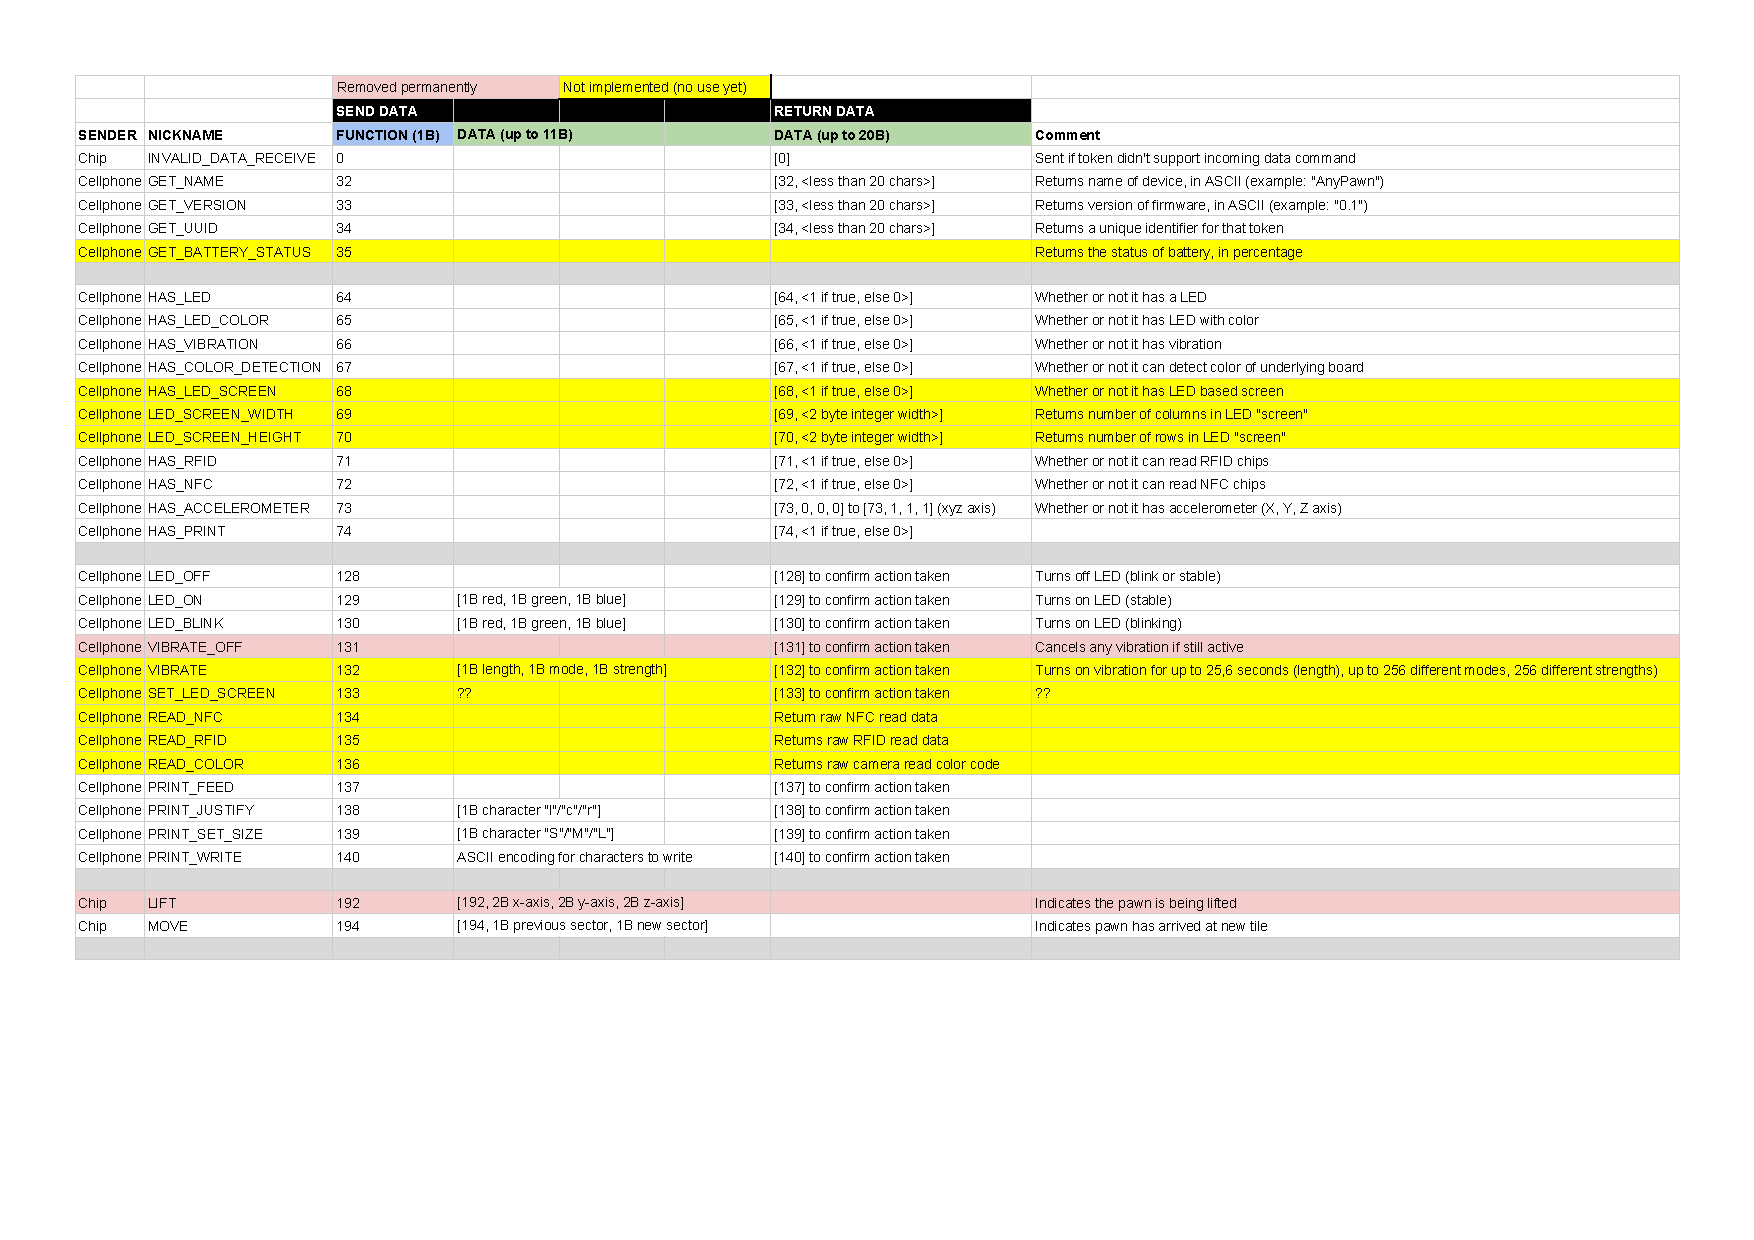
\includepdf[pages=-]{appendix/bluetooth_protocol.pdf}

\chapter{Article: Reflections on AnyBoard} \label{appendix:article}

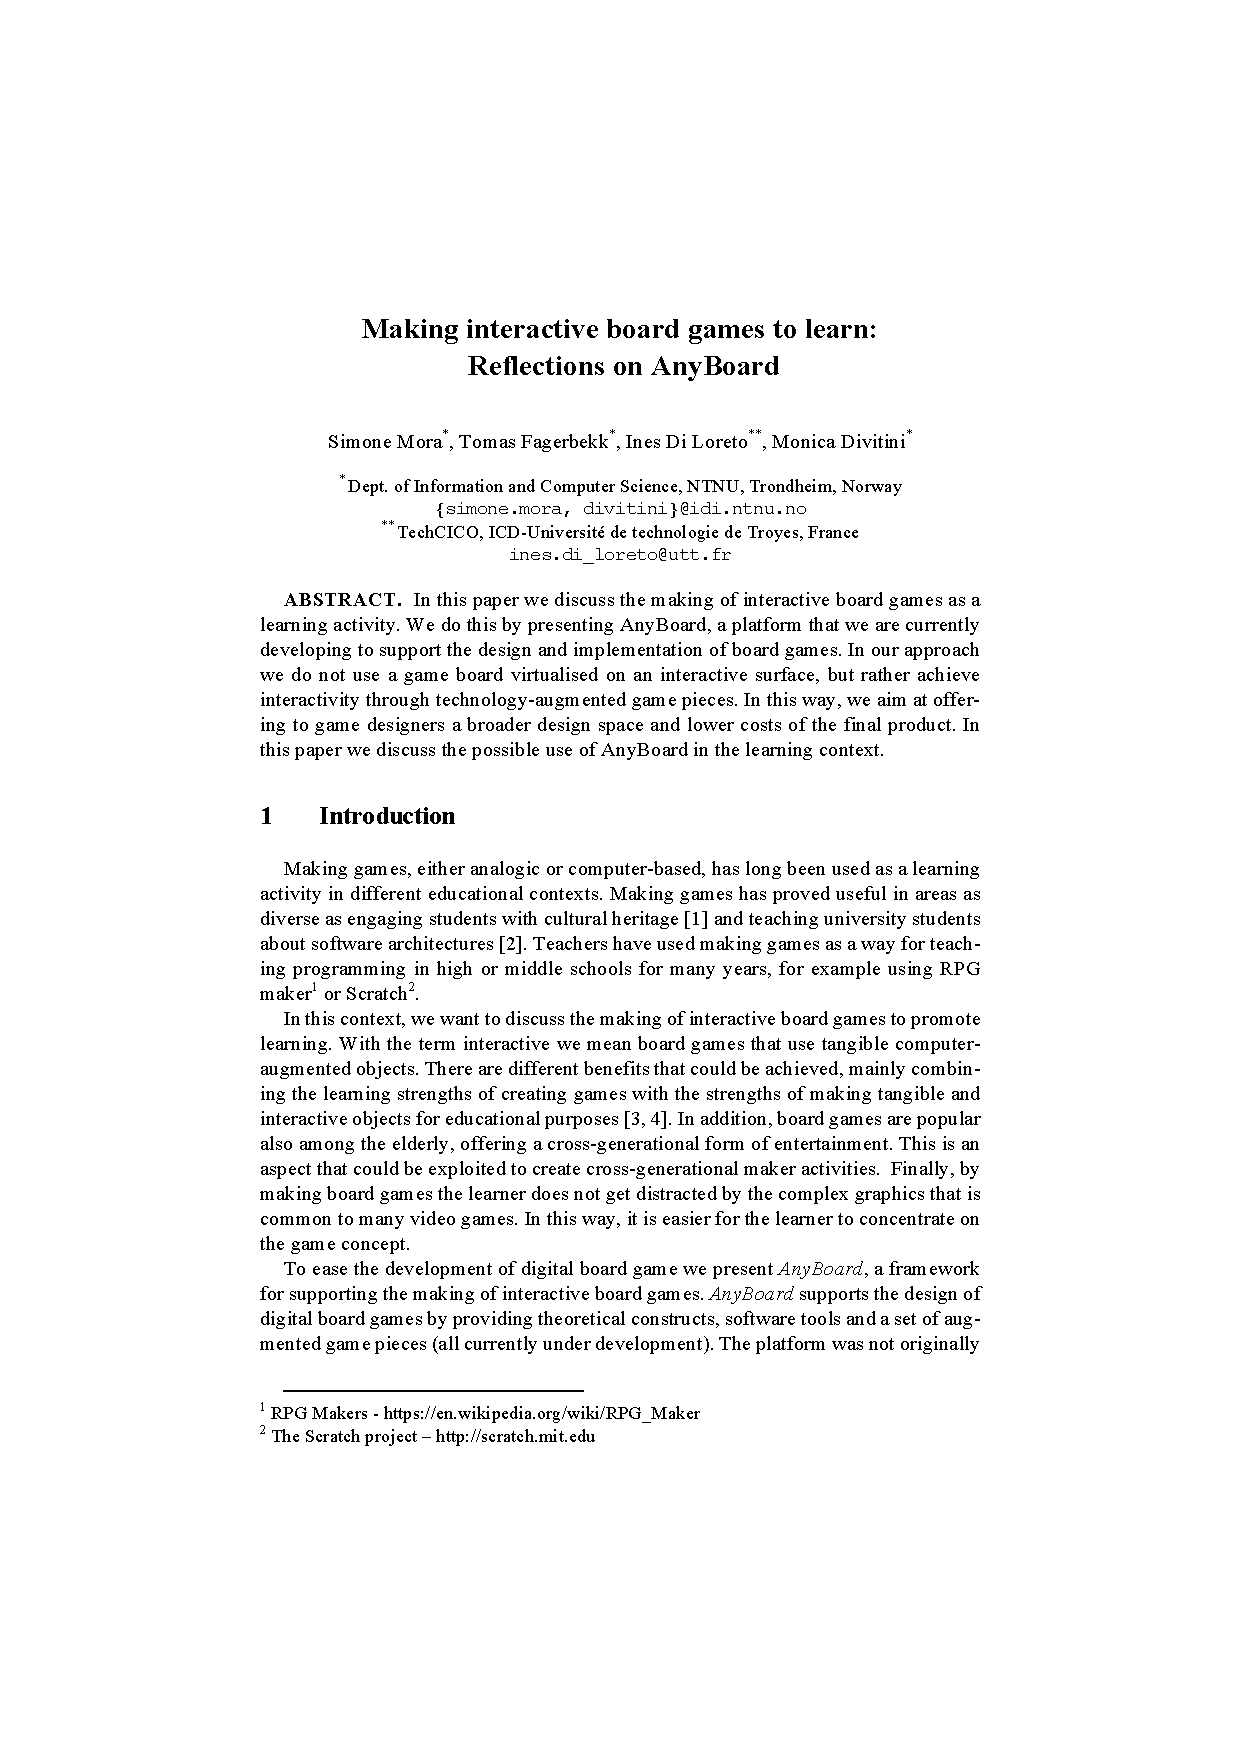
\includepdf[pages=-]{appendix/reflections_anyboard.pdf}

\chapter{AnyBoard Documentation} \label{appendix:doc}

Below is the complete documentation of the AnyBoard library pr. September 2015. This excludes drivers, which is not considered a part of the library. The documentation is also available in interactive format at \href{https://github.com/tomfa/anyboardjs/}{github.com/tomfa/anyboardjs}.

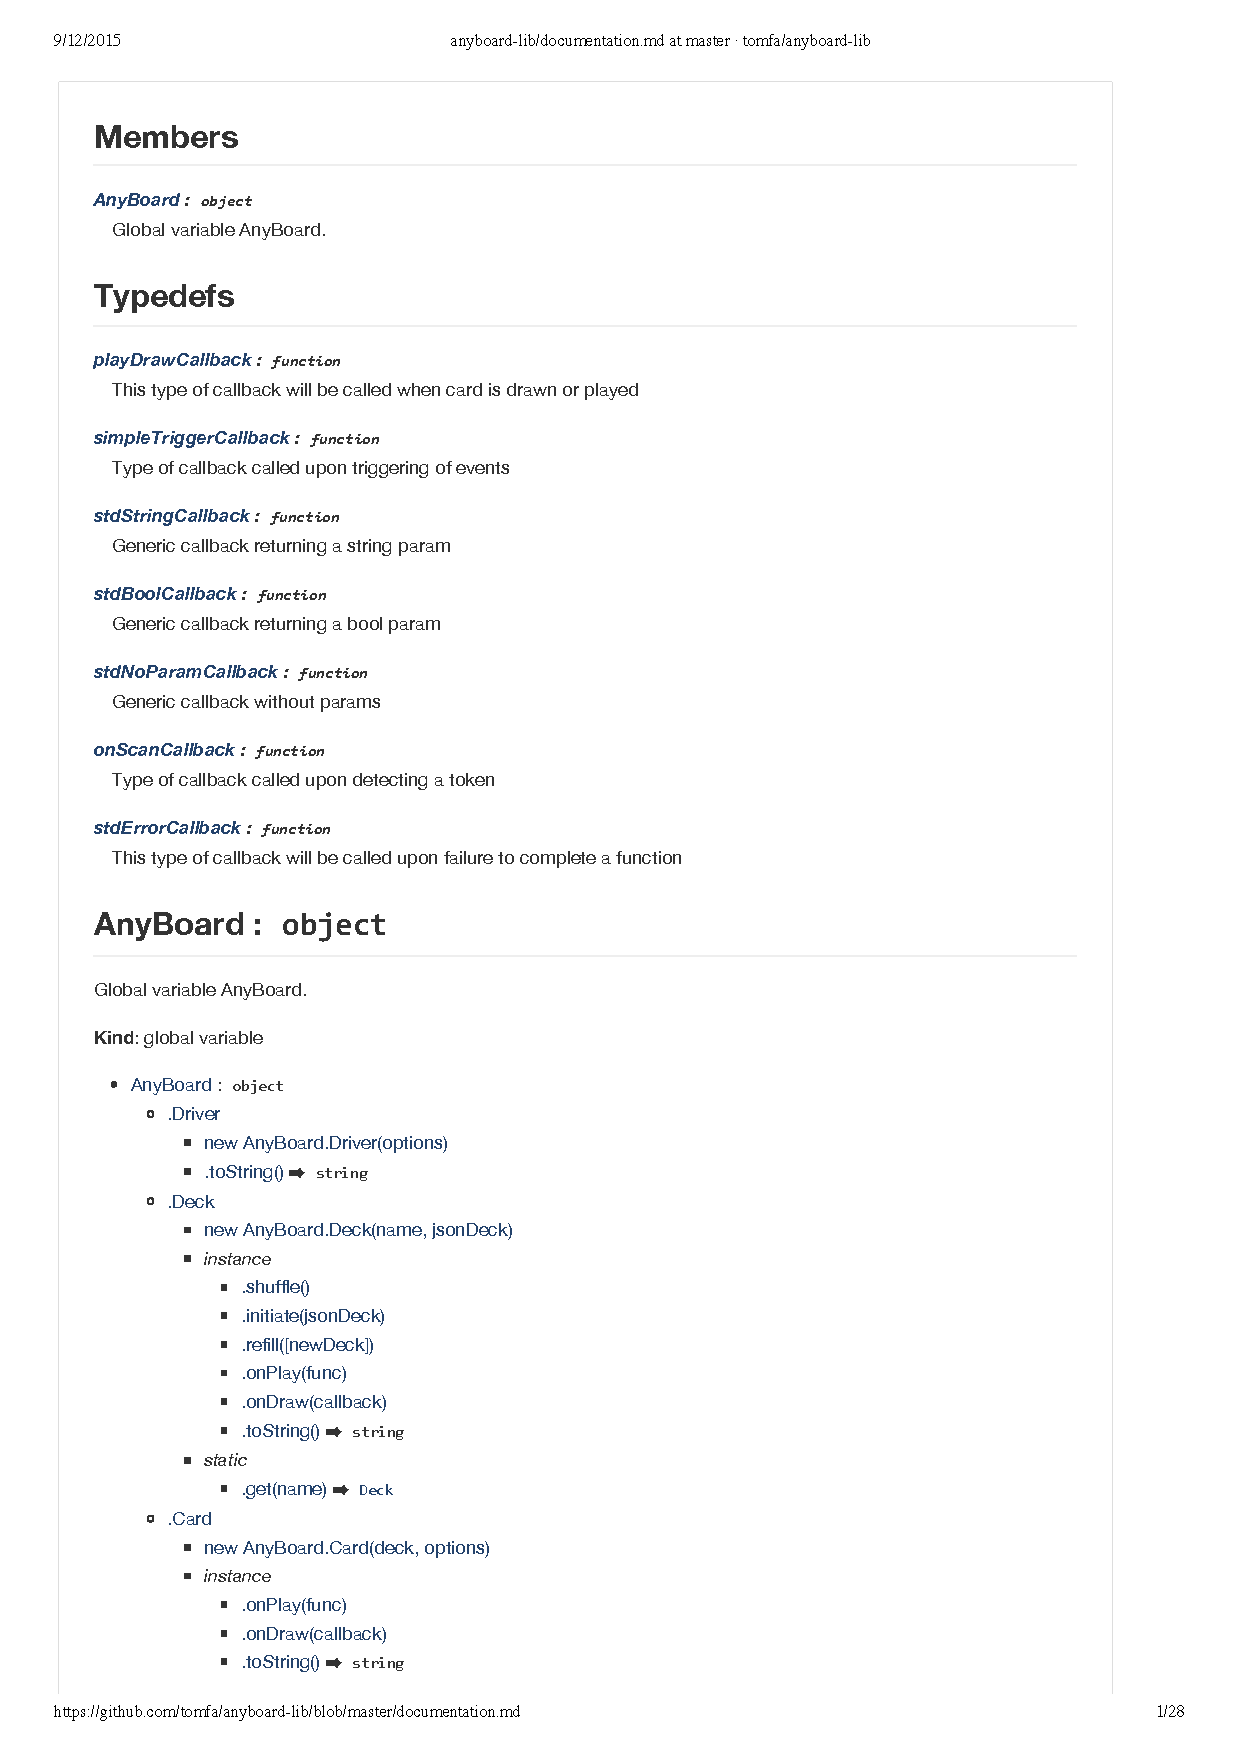
\includepdf[pages=-]{appendix/anyboard-lib_documentation.pdf}
\newpage




\end{document}